\documentclass{scrartcl}
\usepackage[utf8]{inputenc}
\usepackage[english]{babel} % Trennung nach der neuen deutschen Rechtschreibung
\usepackage[utf8]{inputenc}
\usepackage[T1]{fontenc}
\usepackage{lmodern}
\usepackage{subcaption}
\usepackage{chemformula}
\usepackage{placeins}
\usepackage{multirow}
\usepackage{enumitem}
\usepackage{amssymb}
\usepackage{amsmath} % Erweiterte Mathematik-Umgebung
\usepackage{amsfonts} % zusätzliche Mathematik-Schrifttypen (v.a. \mathbb für Mengen)
\usepackage{ulem}
\usepackage{amsthm}
\usepackage{graphics}%soll beim Graphiken einfügen hilfreich sein
\usepackage{graphicx}
\usepackage{wrapfig}%lässt Textumflossene Bildeinbindung zu
\usepackage{epstopdf}%soll eps in pdf umwandeln
\usepackage{placeins}
\usepackage{amsthm}
\usepackage{subcaption}
\usepackage{wrapfig}
\usepackage{hyperref}
\usepackage{ragged2e}

\usepackage[backend=biber, sorting=ynt]{biblatex} %Imports biblatex package
\addbibresource{citation.tex} %Import the bibliography file

\usepackage[a4paper, portrait, margin=2.5cm]{geometry}

\setlength\parindent{0pt}

\begin{document}
\begin{titlepage}
    \begin{center}
        \vspace*{1cm}
        \Huge
        \textbf{Mechanical properties}
        
        \vspace{0.5cm}
        \LARGE
        Advanced Lab Course
        
        \vspace{1.5cm}
        \textbf{Louis-Hendrik Barboutie (020157041C) and Florence Schmerber (0201845640)}
        
        \vspace{1cm}
        Under the supervision of Jorge Alfonso Charry Martinez
        \vfill
        

        
\includegraphics[width=0.4\textwidth]{logo_uni.jpg}
        
        \Large
        17th March 2022
    \end{center}
\end{titlepage}

\clearpage

\tableofcontents

\listoffigures
	
\clearpage

\section{Introduction}
Mechanical properties are physical properties of materials when a certain force is applied on them, like bending or stretching. These properties are essential in engineering, in order to innovate new materials \cite{material}. Such properties are the modulus of elasticity, tensile strength amongst many others. The aim of this experiment is to study the behavior of metals and polymers under tensile and shearing stress, and under 3-point bending. First a tensile test is performed on the different materials, then we will do a shear test on the three metals at out disposal: brass, aluminium and steel. Afterwards, three point bending on these metals will be studied. And finally, we will analyse the stress birefringence of polycarbonate by using a method called photoelasticity.


\section{Theory}
Stress is defined as the force intensity applied on a material, that is the force against a uniformly distributed area. Tensile stress can therefore be defined as \cite{Handout}:
\[\ \sigma= \frac{F_n}{A} \]\ 

with $F_n$ being the deforming force and A the area to which $F_n$ is normal.

 The other form of stress is called shear stress. In this case the deforming force is tangential to the surface of the material, instead of perpendicular to it.
\[\ \tau= \frac{F_t}{A} \]\

Stress can cause deformation, which is measured by strain. Here again, we have two different kinds of strain:
\begin{enumerate}
    \item longitudinal strain: $\epsilon = \frac{\Delta l}{l}$ where l is the lenth of the sample
    \item shearing strain = $\delta = \frac{x}{h}$ where $\delta$ is the change of the angle.
\end{enumerate}

For the case of small deformation, Hooke's law describes the reaction of the material to stress. Point 0 to 1 on figure \ref{fig:Hook} illustrates the region where Hooks law still holds, which means, where the deformation due to stress is still reversible. At  point  2, the body is at its so called limit of elasticity and the according stress is called yield strength. The highest tensile stress at point 3 is called tensile strength. After point 3, the stress seems to decrease, as the material is nearly about to break, which happens at B.
\begin{figure}[h]
\begin{subfigure}{0.5 \textwidth}
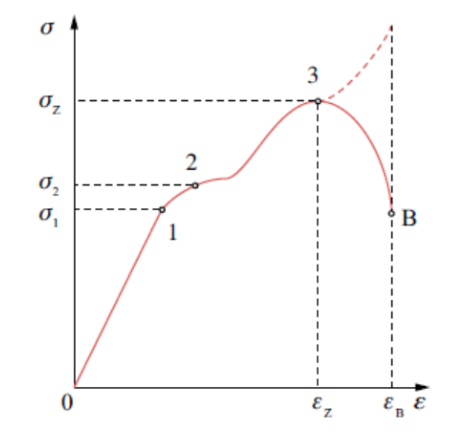
\includegraphics[width=6cm]{Theory and Setup/Screenshot 2022-04-03 121455.png}
\caption{Stress-strain curve for the application of tensile stress to a metal}
\label{fig:Hook}
\end{subfigure}
\begin{subfigure}{0.5 \textwidth}
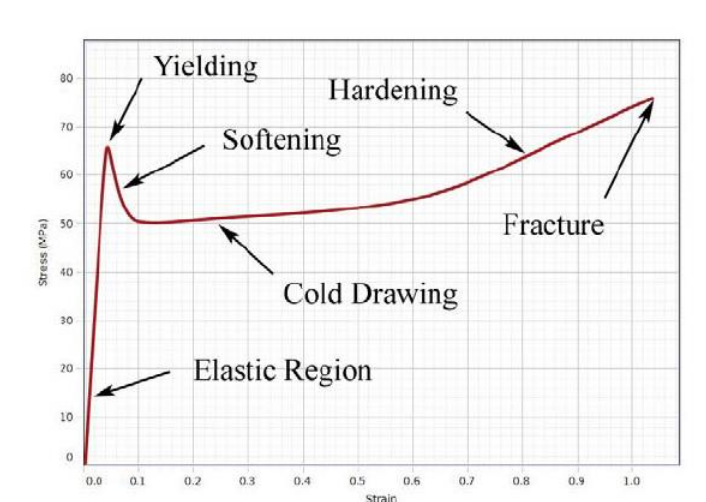
\includegraphics[width=7cm]{Theory and Setup/Screenshot 2022-04-03 123306.png}
\caption{Stress-strain curve for plastic}
\label{fig:polymers}
\end{subfigure}
\end{figure}


Hooks law states that: 
\begin{align}
    \sigma &= E\epsilon \\
     \tau &= G\delta
\end{align}
The proportional constants E and G are called Young's modulus and shear modulus respectively.

On the other hand, polymers behave differently than metals (see figure \ref{fig:polymers}). First stress builds up until the neck of the polymer is build (the yielding point). This neck forms by the disentangling of the polymer chains. After that, the polymer seems to be stretched out until it breaks.\vspace{0,5cm}

When a force is applied on a sample to increase its length, both the lateral and and perpendicular length changes. This deformation is described by the the Poisson ratio $\mu$:
\[\ \mu = \frac{\frac{\Delta d}{d}}{\frac{\Delta l}{l}} \]\

Additionally, the volume changes too when we apply a tensile force. \vspace{0,5cm}

Through a three point bending experiment, the flexural elastic modulus, denoted E, can be determined. The following formula for rods with a circular cross-section will be used:
\[\ h = \frac{l^3}{12 \pi R^4 E}F \]\

With h being the deflection of the rod, l the length, $F$ the force applied, $R$ the radius of the rod.

For the last part we will determine the stress distribution in birefringent plastic using photoelasticity. "Birefringence is the optical property of a material having a refractive index that depends on the polarization and propagation direction of light"\cite{birefringence}. Inside  the material, light of different polarizations travels with different velocities, which will create constructive of destructive interference and will create these fringes. 

\section{Experimental setup}

\begin{wrapfigure}{r}{0.4\textwidth}
    \centering
    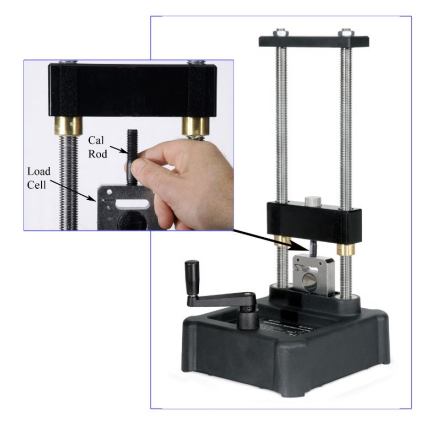
\includegraphics[width=6cm]{Theory and Setup/Screenshot 2022-04-03 104556.png}
    \caption{Setup for calibration}
    \label{fig:cal}
\end{wrapfigure}
Today we will be using the same apparatus for every measurement. It is composed of a crosshead that can be moved through a crank handle. We can install different pieces onto the the load cell depending on the desired measurement. For the first part, the calibration, a calibration rod will be installed(see figure \ref{fig:cal}). For the tensile test, the sample will be screwed between the load cell and the cross head, then the crosshead will be cranked up until it breaks. The software that we will be using throughout the experiment, will record all the necessary data. In order to do the shear test, the material shear accessory is mounted onto the loading cell and secured by two screws. The vertical piece (shear front) slides up and the metal sample is put into the device. A shearing force is applied onto the metal, until it breaks. The shear strength will be measured for each material and compare them with each other.Next, to perform the three-point bending test, the metal rods are placed centered on the anvils, while a third one puts a downward force in the middle of the rod. For the last part, the bending accessory is install, which will but a compression force onto a clear polycarbonate. Two polarizing sheets are placed on each side of the apparatus. When illuminated by a source of light, fringes on the plastic can be seen and are analysed for this part.

\section{Results}

\subsection{Calibration}
The calibration is necessary for the accuracy of the  measurement. Do to so, the calibration rod is placed into the load cell. We have to make sure that the knurled cap stays loose, not creating any force. Then, we load and unload the system by increasing and decreasing the applied force between 10 N and 20 N to "seat" the sample. When this is done, we increase the force up to 100 N and stop recording. Now we have a pre-load of 100 N, because the measurements under amount of force are not linear and thus gives us better data. Then, we increase the force up to 7000 N. As a result we get a linear curve (see graph \ref{fig:calibration}). We will substract the data from the calibration for every recorded tensile test to ensure a precise result.
\begin{figure}[h]
    \centering
    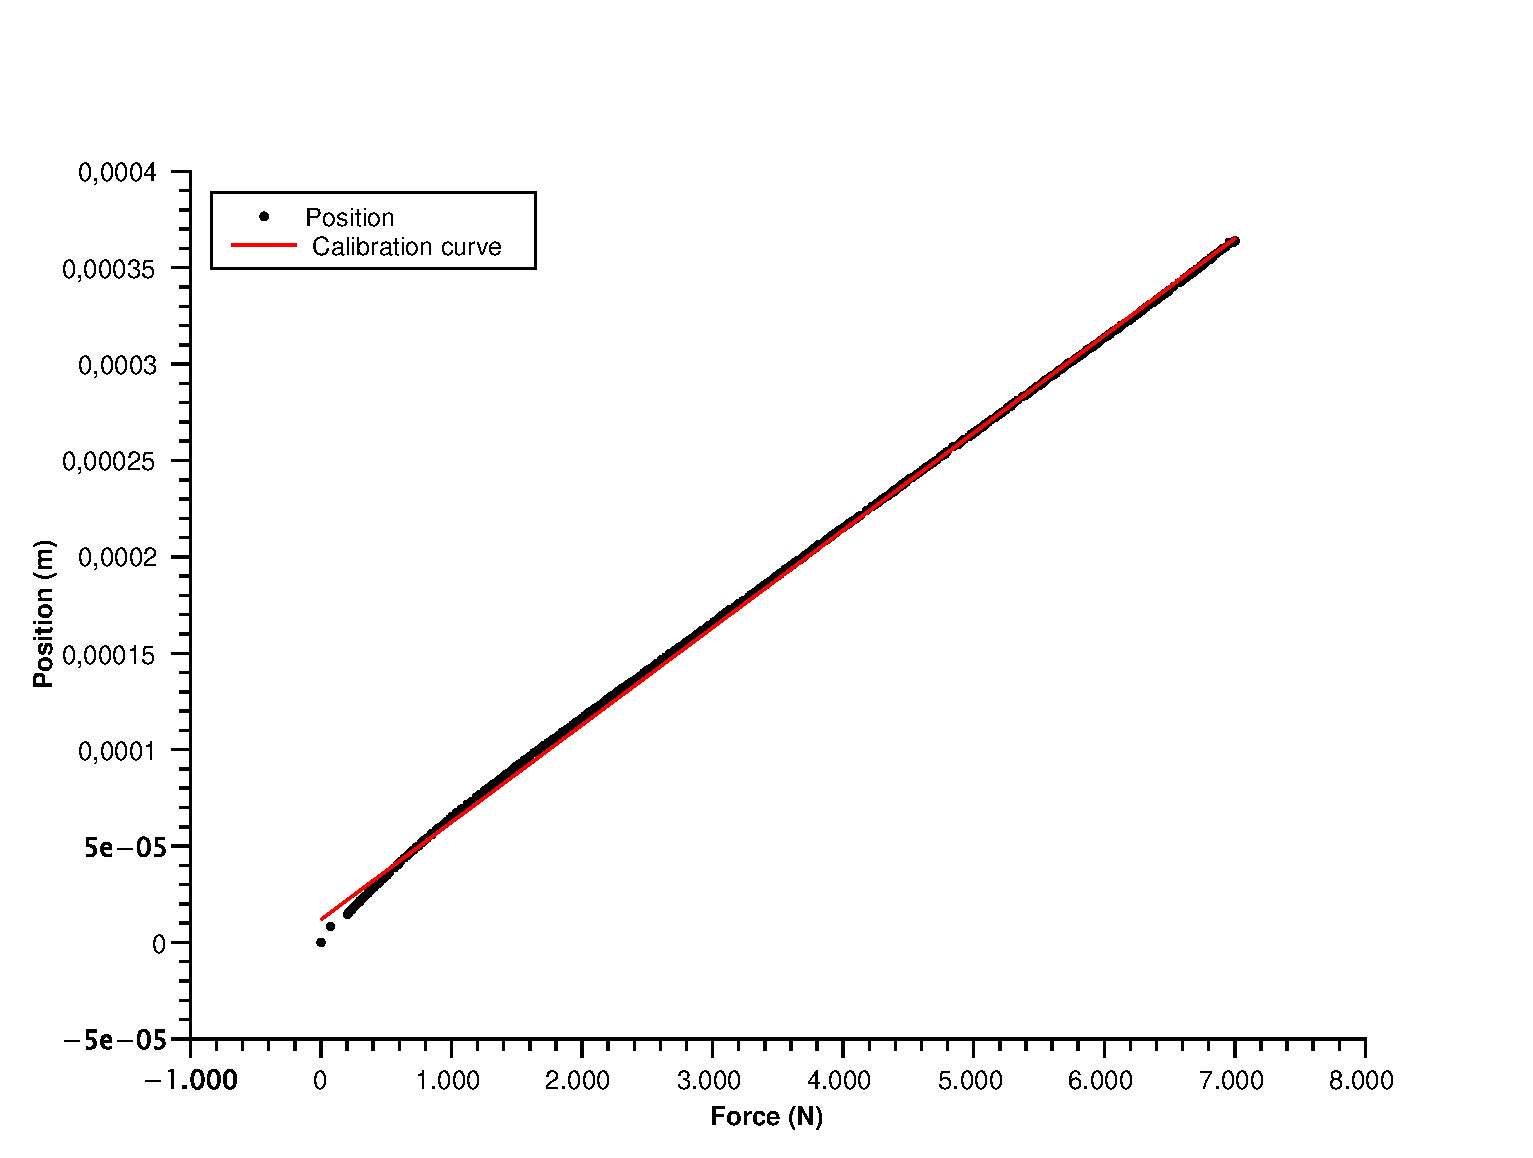
\includegraphics[width=0.7\textwidth]{Calibration/CalibrationCurve.eps}
    \caption{Calibration curve for the tensile test}
    \label{fig:calibration}
\end{figure}

We get a linear fit for the data: 
\begin{equation}
    x = aF+b
\end{equation} 

With $a=5,0481501450683 \cdot 10^{-8} \ \text{mN}^{-1} $ and $b=1,1863736566168 \cdot 10^{-5} \ \text{m}$ given by qtiPlot, We can then use the calibration curve to correct the data on the position with the following relationship: \begin{equation}
    x' = x-(aF+b)
\end{equation}

\subsection{Tensile test}

\subsubsection{Metals}

We measure the dimensions of the test samples: the diameter $d$, and the length $l$. The diameter and length of all the samples are the same. We get : 
\begin{align}
d &= (3.40 \pm 0.05) \cdot 10^{-3} \ \text{m} \\ l &= (89.00 \pm 0.05) \cdot 10^{-3} \ \text{m} 
\end{align} 

We can then determine $A$, the area of the surface to which the applied force is normal. In our case it is a disk, and: \begin{equation}
    A = \pi \left( \frac{d}{2} \right)^2 \approx 9.08 \cdot 10^{-6} \ \text{m}^2
\end{equation}

Using the recorded data, we can plot the force as a function of change in position (i.e. elongation of the sample) and stress as a function of strain. If we make a linear fit in the region where the sample undergoes small deformation, Young's modulus and the shear modulus are given by the slope of the fits for stress(strain) and force(position) respectively.

\begin{figure}[!ht]
    \begin{subfigure}{0.49\textwidth}
        \centering
        \resizebox{\textwidth}{!}{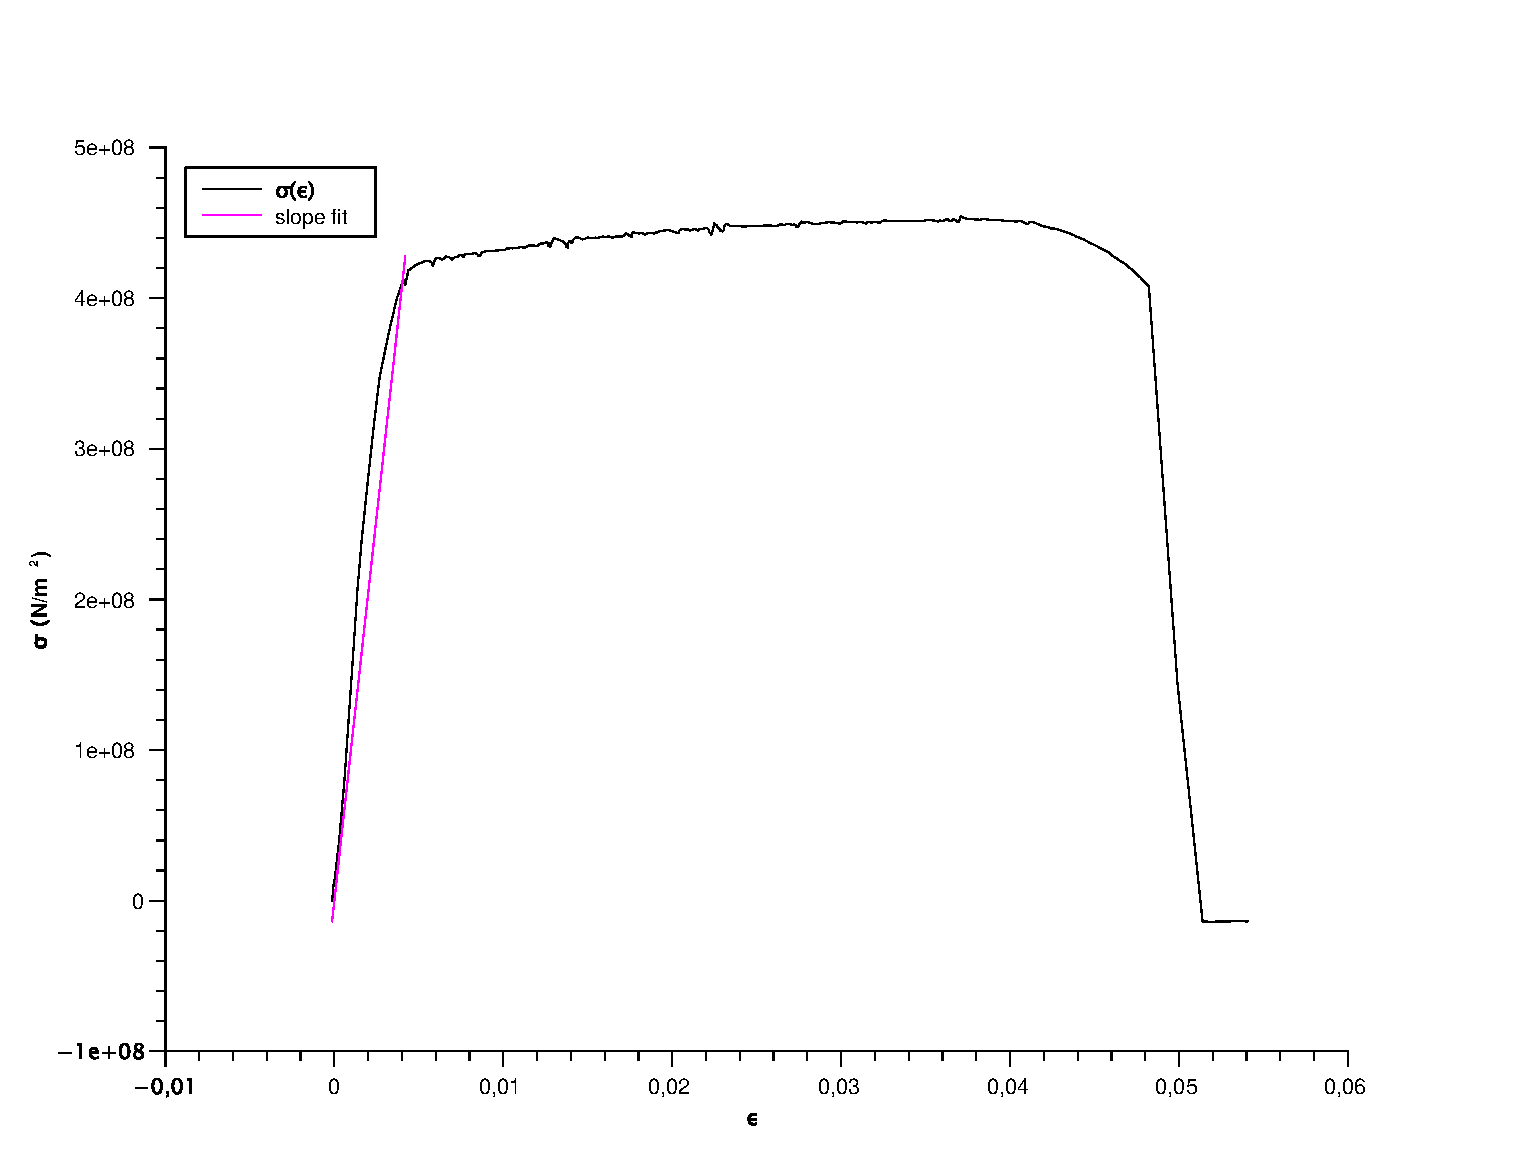
\includegraphics{Tensile/TensileBrassSigma.eps}}
        \caption{$\sigma ( \epsilon)$ for brass}
        \label{fig:brass_sigma}
    \end{subfigure}
    \begin{subfigure}{0.49\textwidth}
        \resizebox{\textwidth}{!}{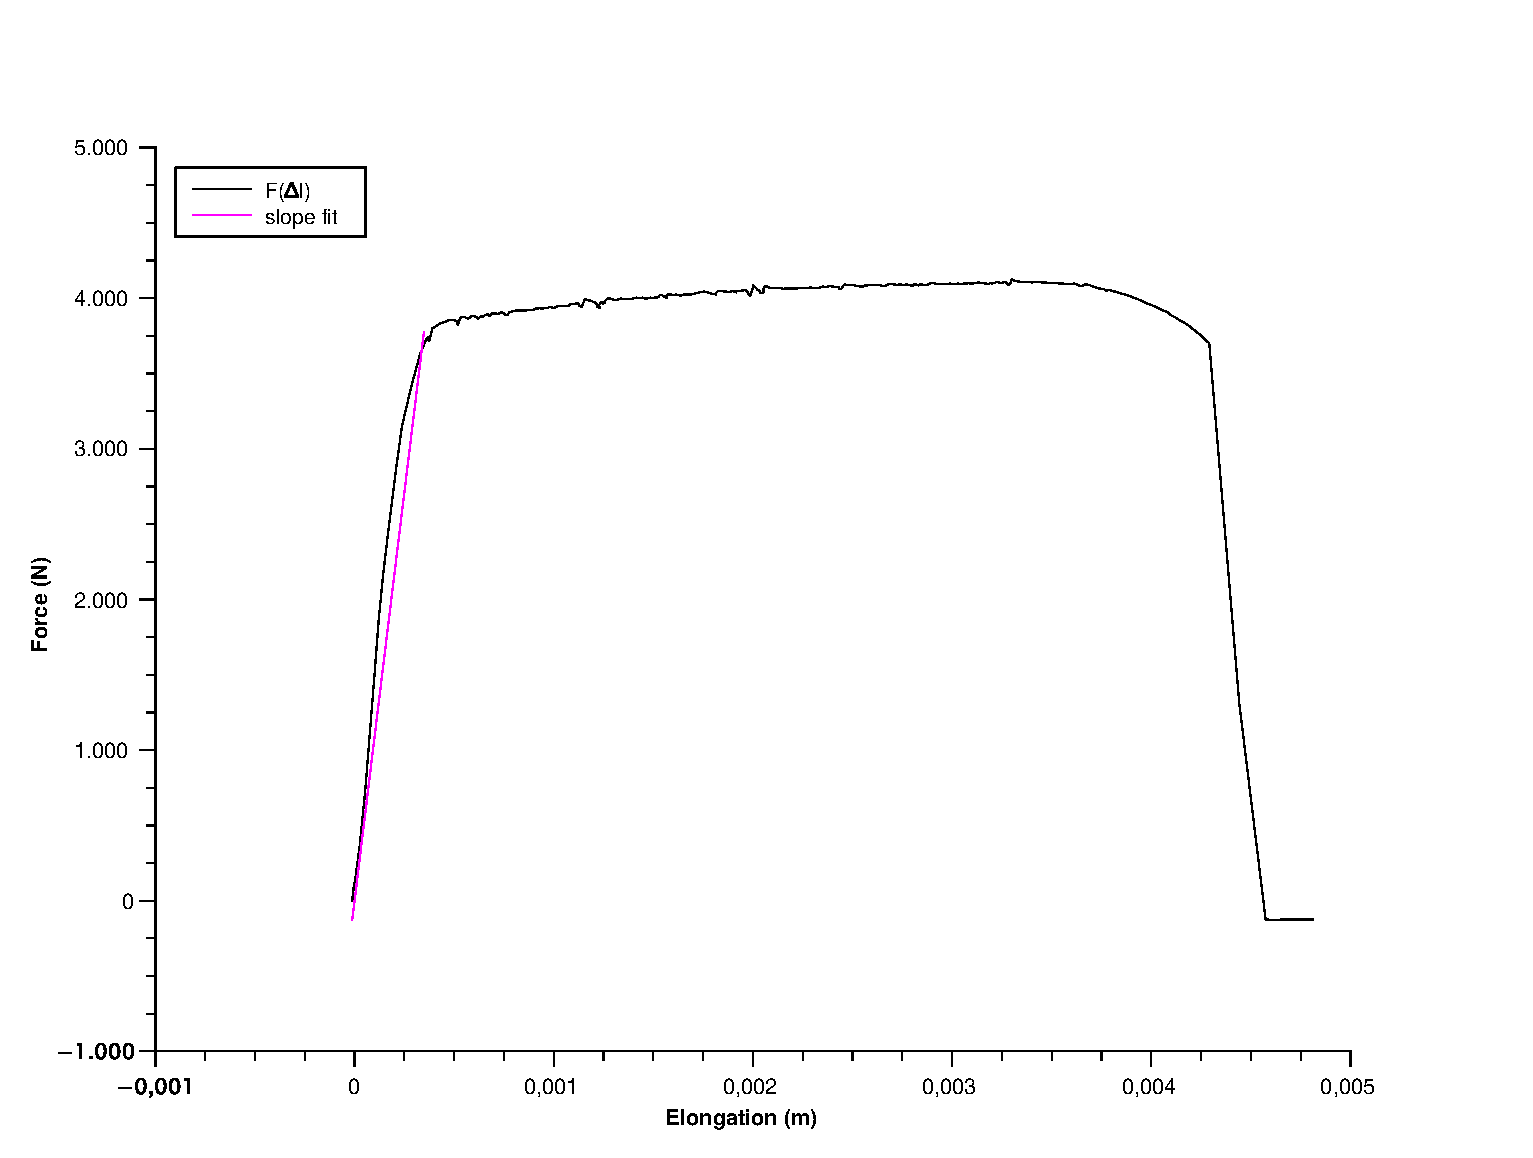
\includegraphics{Tensile/TensileBrassForce.eps}}
        \caption{F($\Delta l$) for brass}
        \label{fig:brass_Force}
    \end{subfigure}
    \caption{Tensile test of Brass}
    \label{fig:tensileBrass}
\end{figure}

\begin{figure}[!ht]
    \begin{subfigure}{0.49\textwidth}
        \centering
        \resizebox{\textwidth}{!}{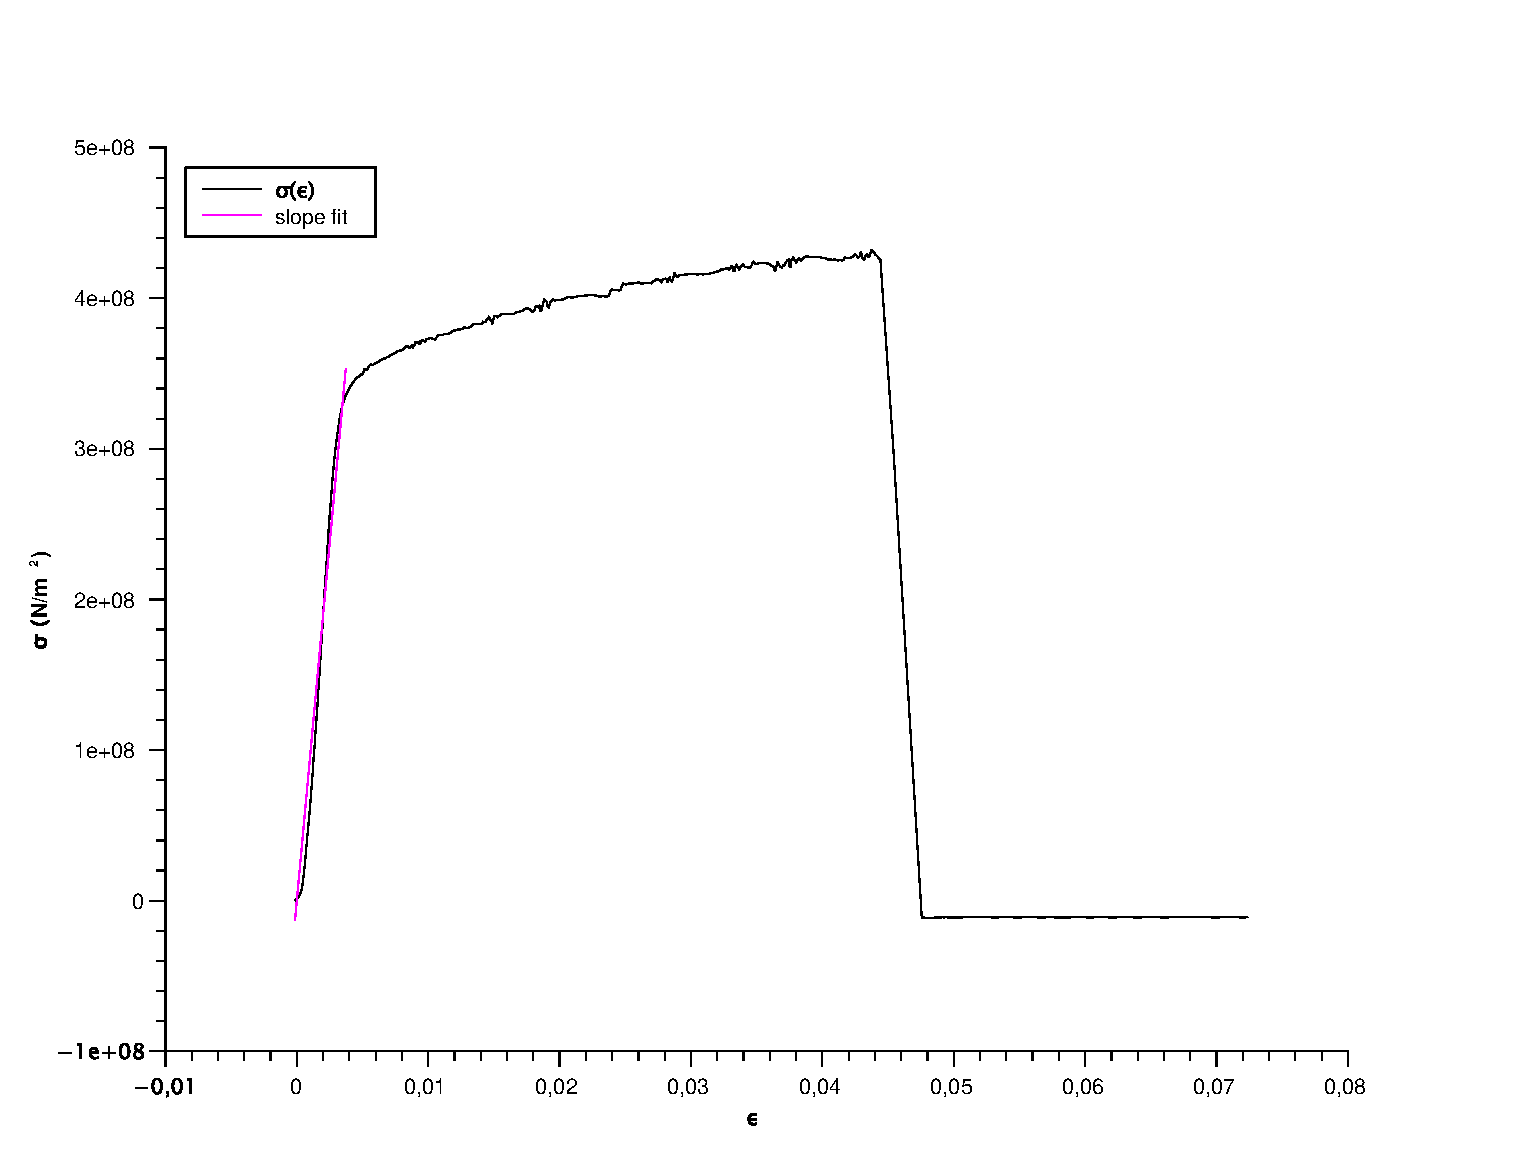
\includegraphics{Tensile/TensileAluSigma.eps}}
        \caption{$\sigma ( \epsilon)$ for Aluminium}
        \label{fig:alu_sigma}
    \end{subfigure}
    \begin{subfigure}{0.49\textwidth}
        \resizebox{\textwidth}{!}{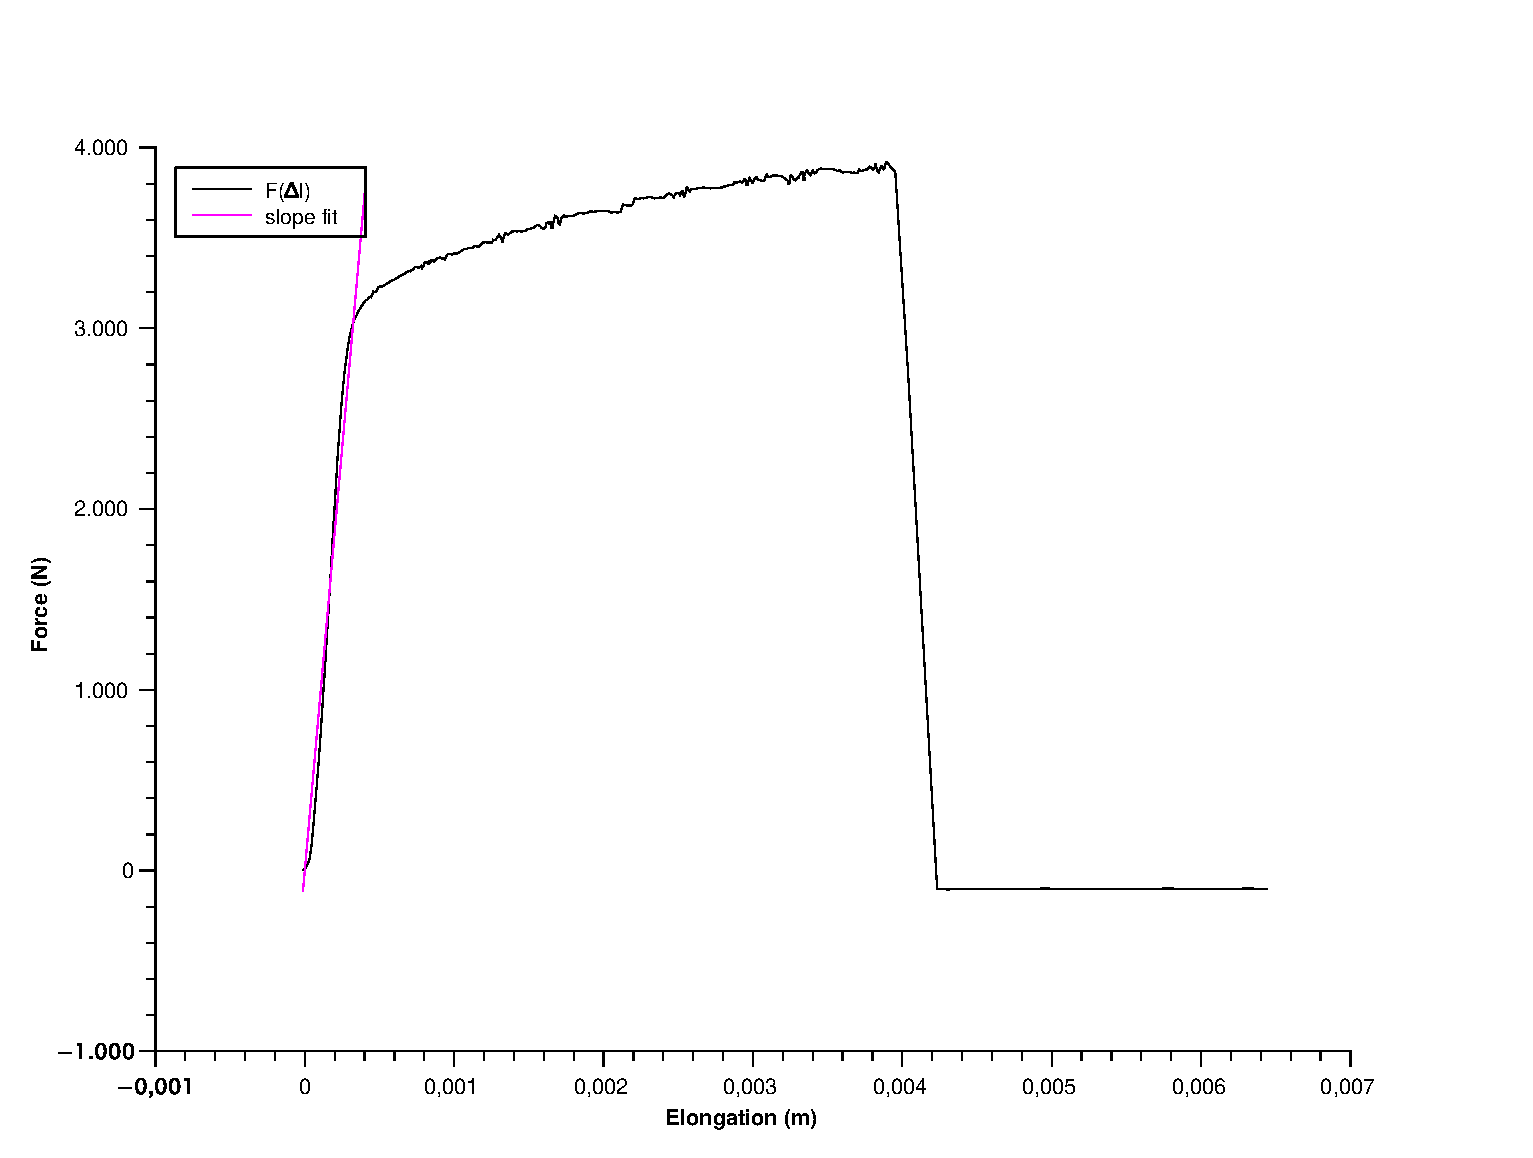
\includegraphics{Tensile/TensileAluForce.eps}}
        \caption{F($\Delta l$) for Aluminium}
        \label{fig:alu_Force}
    \end{subfigure}
    \caption{Tensile test of Aluminium}
    \label{fig:tensileAlu}
\end{figure}

\begin{figure}[!ht]
    \begin{subfigure}{0.49\textwidth}
        \centering
        \resizebox{\textwidth}{!}{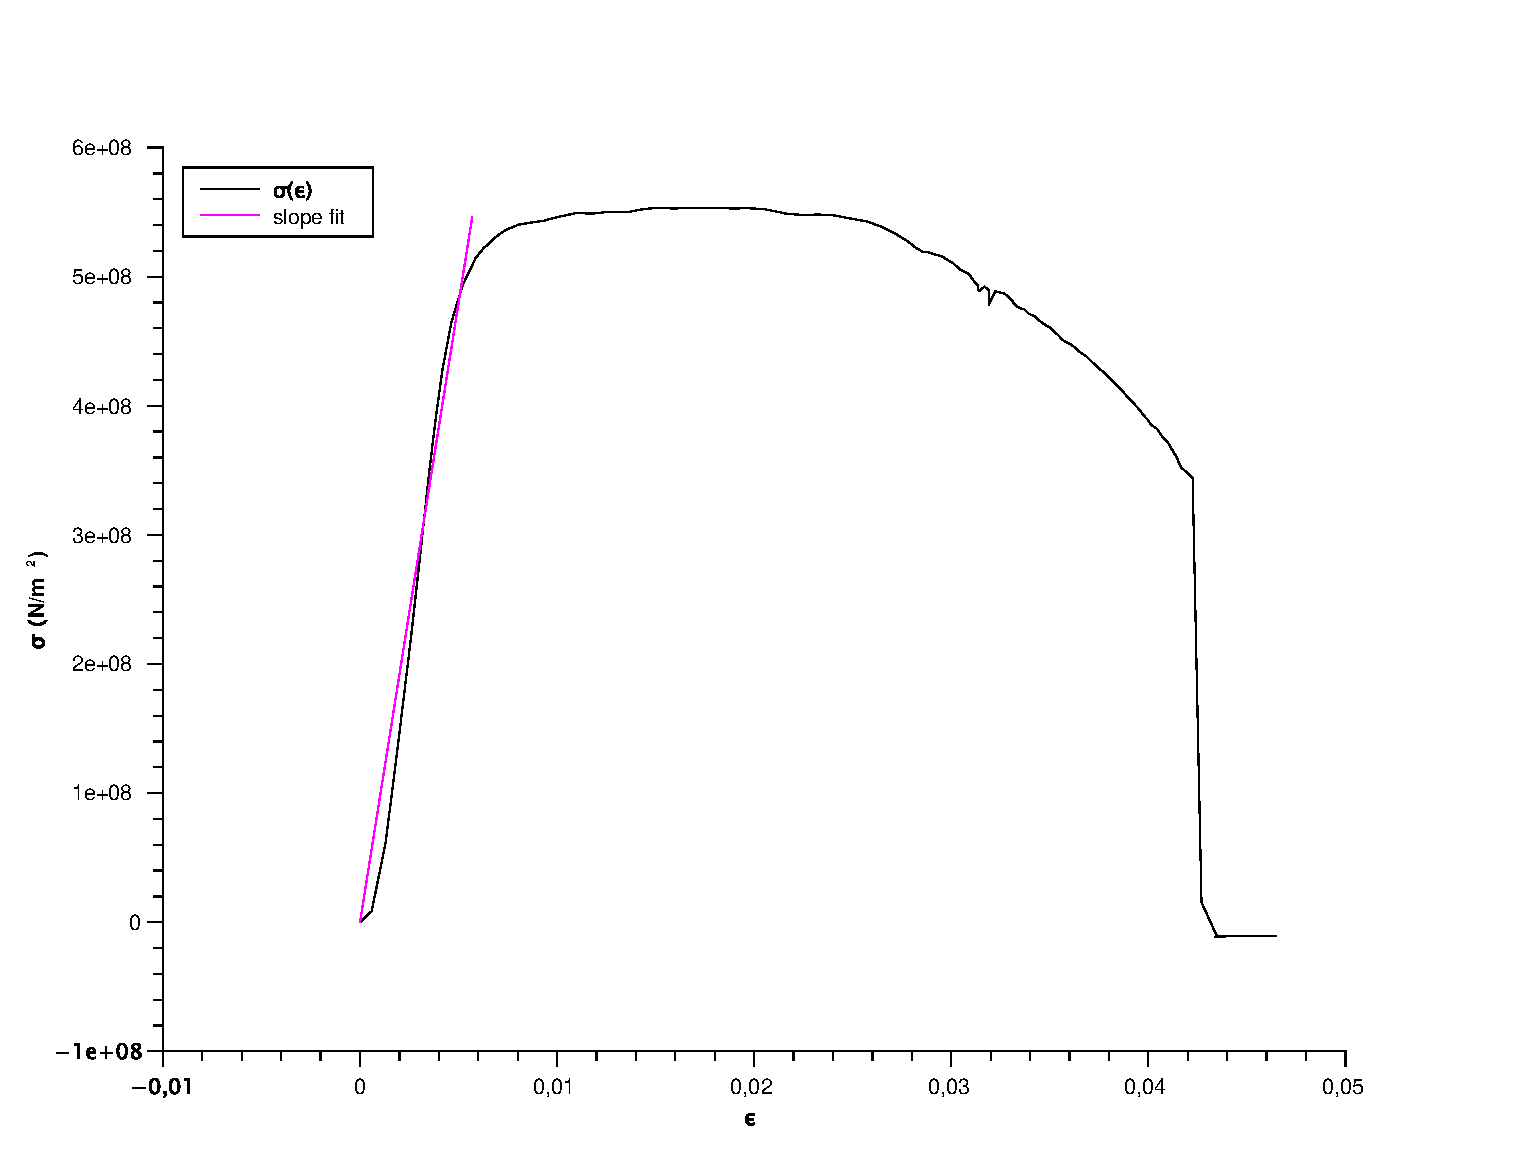
\includegraphics{Tensile/TensileSteelSigma.eps}}
        \caption{$\sigma ( \epsilon)$ for Steel}
        \label{fig:steel_sigma}
    \end{subfigure}
    \begin{subfigure}{0.49\textwidth}
        \resizebox{\textwidth}{!}{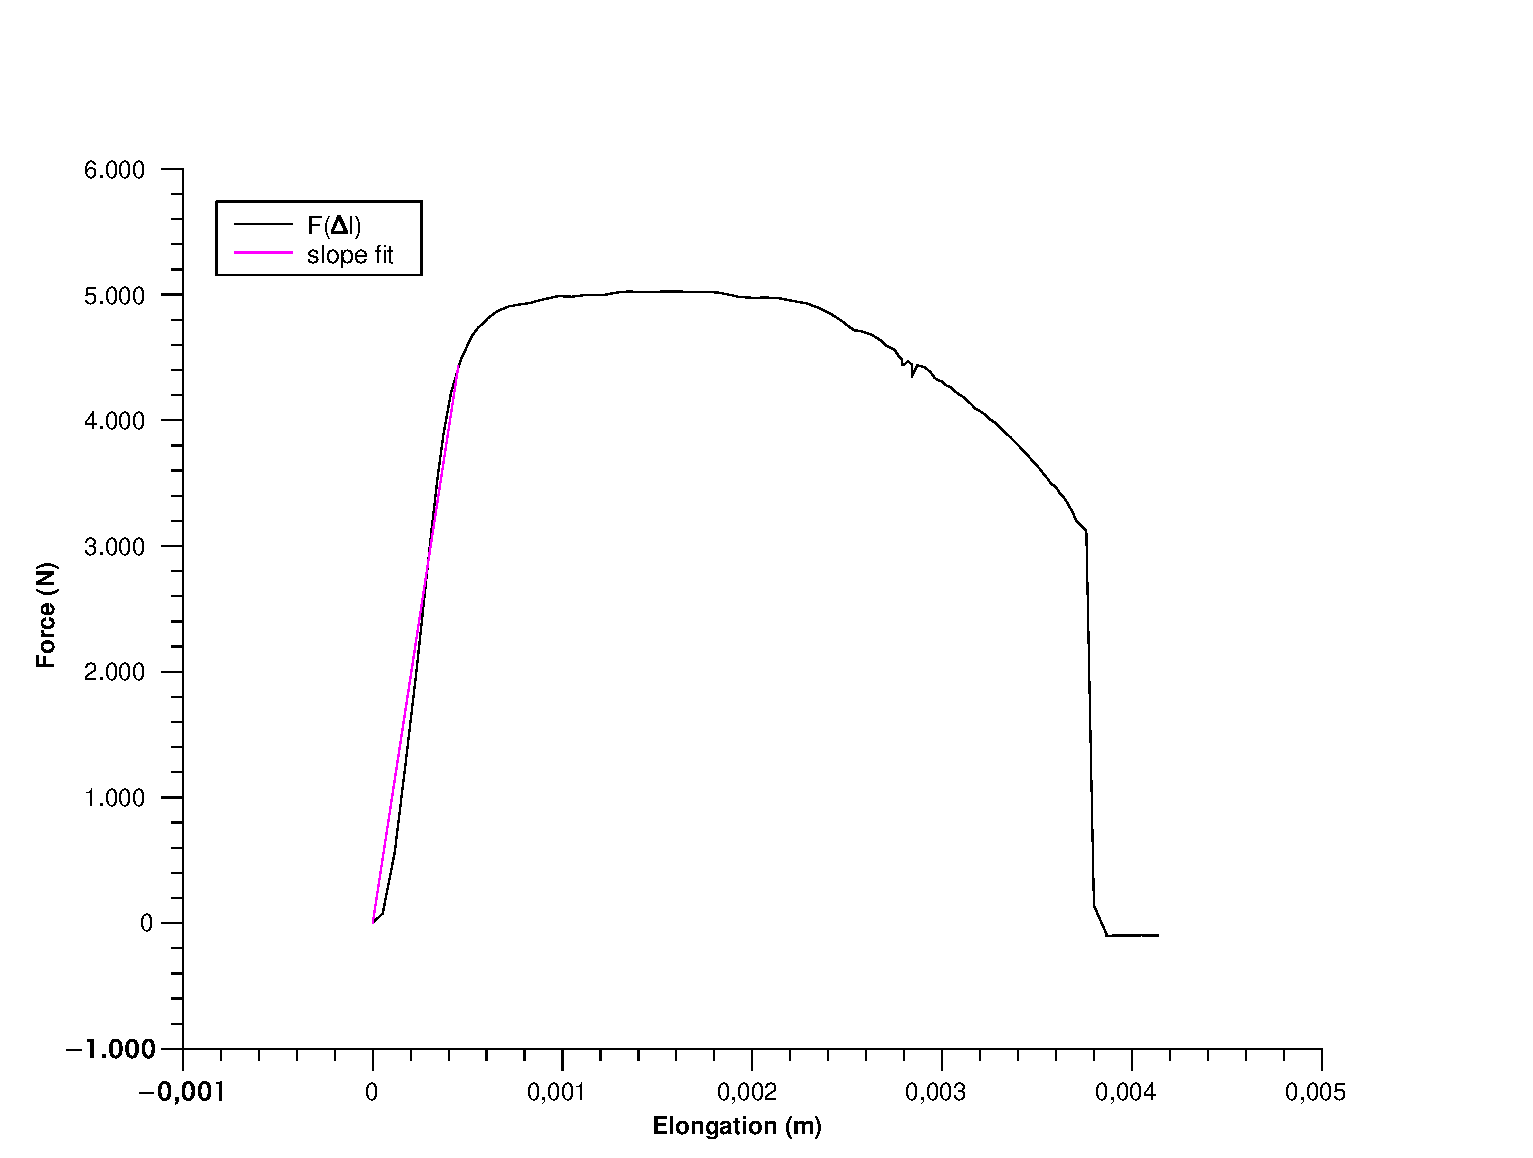
\includegraphics{Tensile/TensileSteelForce.eps}}
        \caption{F($\Delta l$) for Steel}
        \label{fig:steel_Force}
    \end{subfigure}
    \caption{Tensile test of Steel}
    \label{fig:tensileSteel}
\end{figure}

\begin{figure}[!ht]
    \begin{subfigure}{0.49\textwidth}
        \centering
        \resizebox{\textwidth}{!}{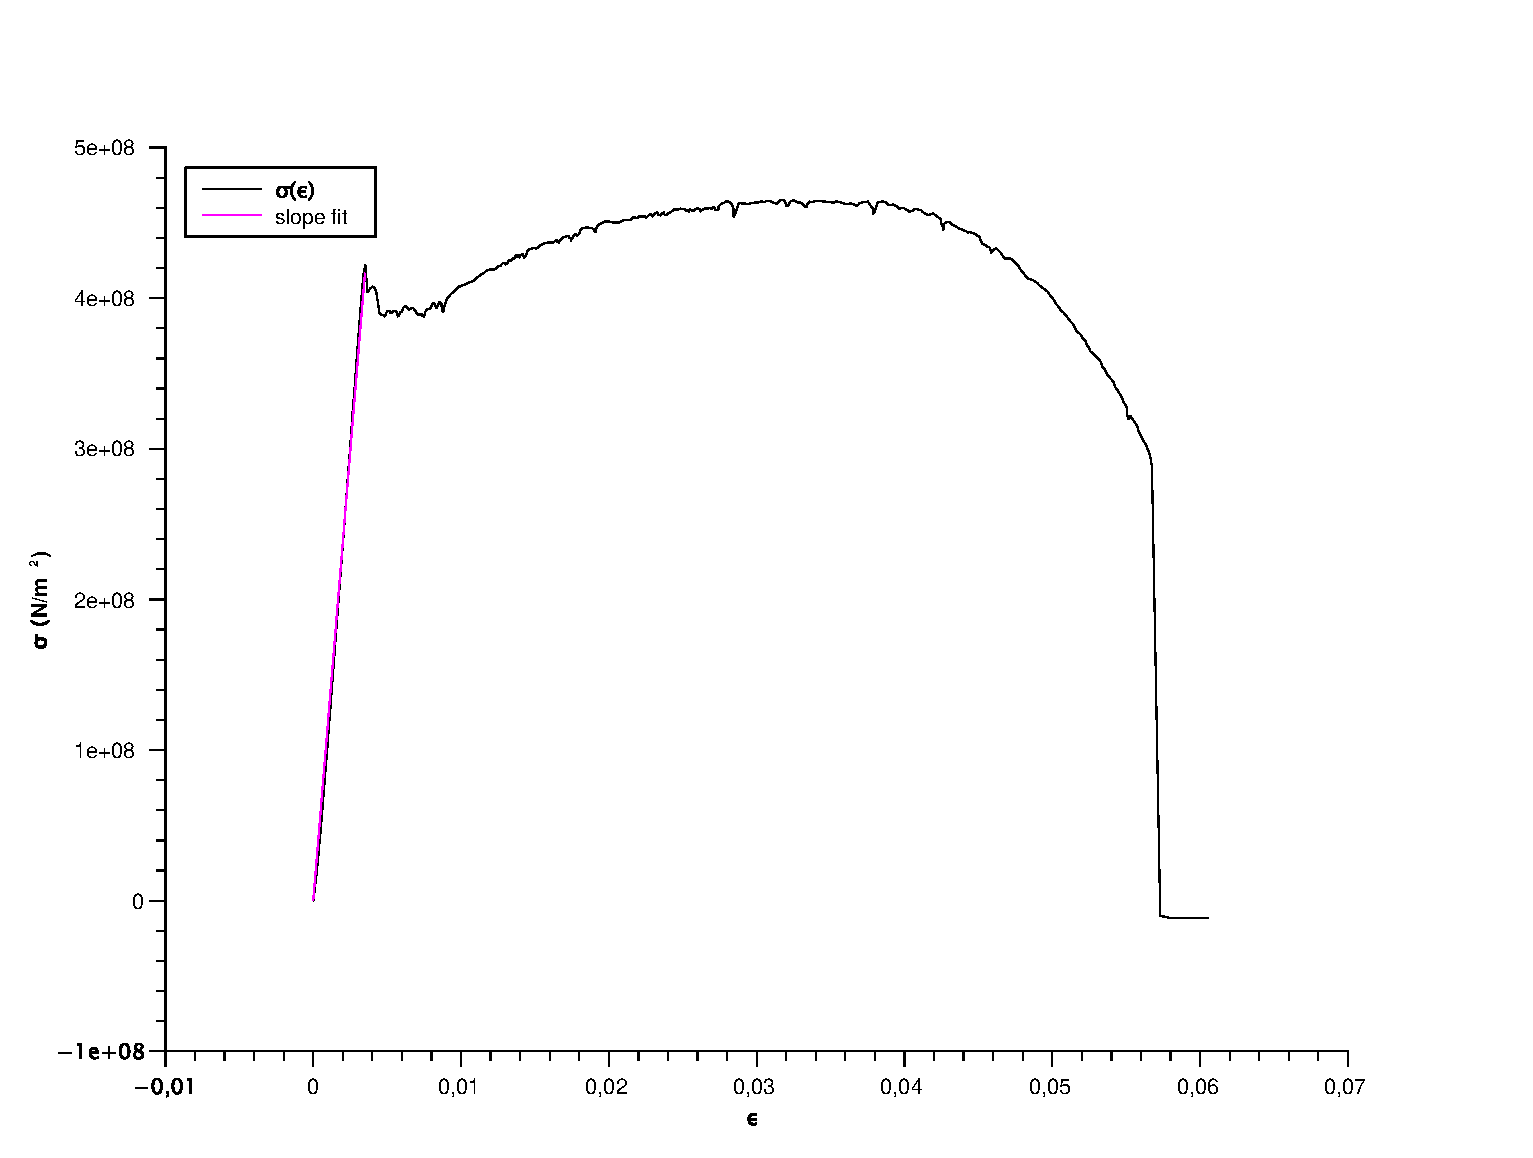
\includegraphics{Tensile/TensileSteelAnnealedSigma.eps}}
        \caption{$\sigma ( \epsilon)$ for brass}
        \label{fig:steelAnnealed_sigma}
    \end{subfigure}
    \begin{subfigure}{0.49\textwidth}
        \resizebox{\textwidth}{!}{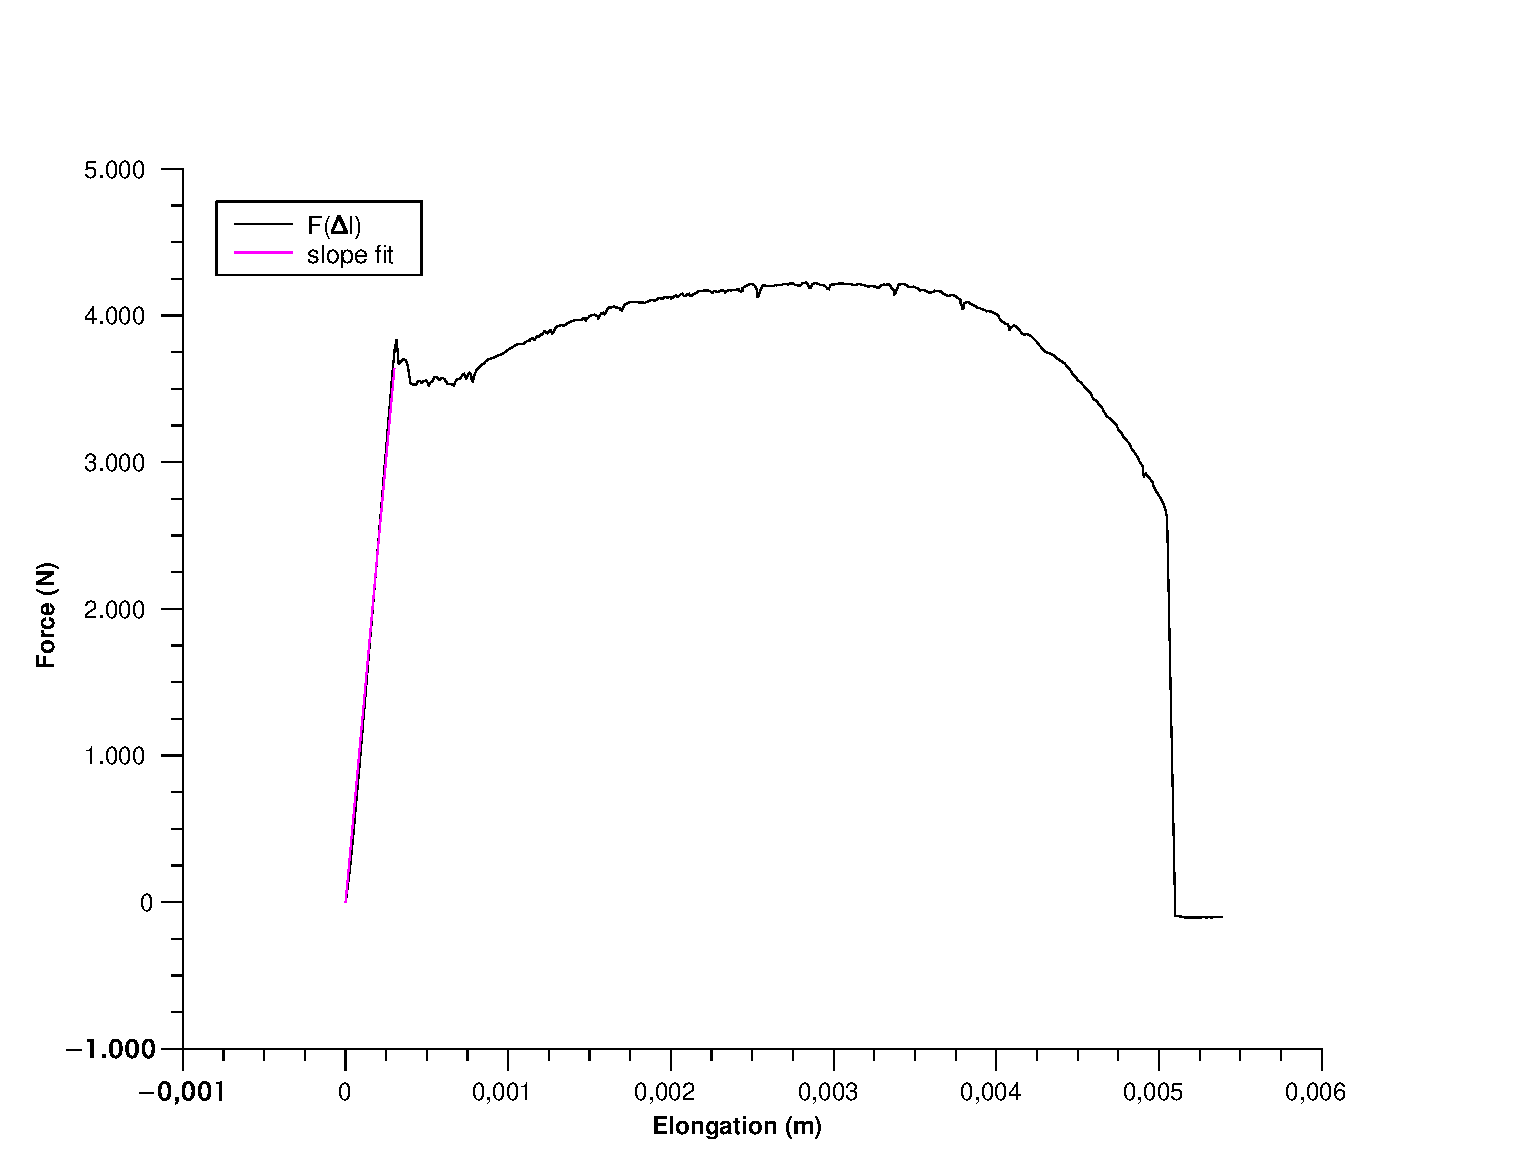
\includegraphics{Tensile/TensileSteelAnnealedForce.eps}}
        \caption{F($\Delta l$) for brass}
        \label{fig:steelAnnealed_Force}
    \end{subfigure}
    \caption{Tensile test of annealed Steel}
    \label{fig:tensileSteelAnnealed}
\end{figure}
\FloatBarrier

\begin{figure}[h]
    \centering
    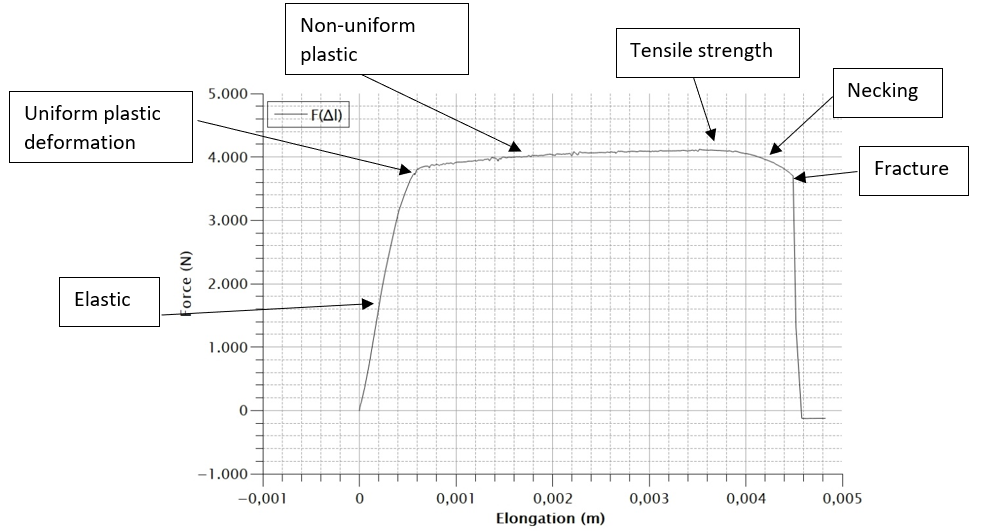
\includegraphics[width=0.7\textwidth]{Tensile/annotated_brass.png}
    \caption{Regions for a metal sample (here brass)}
    \label{fig:annotated_metal}
\end{figure}
\FloatBarrier

It is no surprise that these curves have the same appearance, since $\epsilon$ is just a rescaled $\Delta l$, and $\sigma$ is a rescaled $F$. The slope coefficients give us the stiffness $k$, with $F(\Delta l)$, and Young's modulus $E$ with $\sigma(\epsilon)$. The values of these constants can be found in table~(\ref{tab:youngMod_Stiffness}). 

The overall shape of these curves is close to what we expected. The materials all begin to elongate elastically (this is the linear region in the $\sigma(\epsilon)$ graphs), followed by an elastic, but non-linear elongation, and then a constriction until the breaking point (see figure \ref{fig:annotated_metal} for the annotated regions for a metal sample). Annealed steel has another interesting feature: it undergoes a yielding, softening and cold drawing phase right after the linear elongation. The Aluminium sample also doesn't seem to undergo constriction; during the experiment, it seemed that a neck was forming, but the sample broke before it could finish forming. This is in contrast to the rest of the samples, which broke along a clean plane.

\begin{table}[!ht]
    \centering
    \begin{tabular}{c|c|c}
        Material & $E \ (10^{10} \ \text{Nm}^{-2})$ & $k \ (10^{6} \ \text{Nm}^{-1})$ \\ \hline
        Brass & 10.19 & 10.85 \\
        Aluminium & 9.48 & 9.35 \\
        Steel & 9.59 & 9.82 \\
        Annealed Steel & 11.91 & 12.13 
    \end{tabular}
    \caption{Experimental values of Young's modulus $E$ and stiffness $k$ of various material samples}
    \label{tab:youngMod_Stiffness}
\end{table}

We can also determine the tensile strength, ie. the maximum force exerted on the sample, as well as the maximum elongation.

\begin{table}[!ht]
    \centering
    \begin{tabular}{c|c|c}
        Material & max. force (N) & max. elongation ($10^{-3}$ m) \\ \hline
        Brass & 4124 & 4.3 \\
        Aluminium & 3920 & 4.0 \\
        Steel & 5025 & 3.8 \\
        Annealed Steel & 4225 & 5.1 
    \end{tabular}
    \caption{Maximum elongation and maximum force of various material samples}
    \label{tab:tensile_maxForce_maxElongation}
\end{table}

\subsubsection{Polymers}

In the previous section, we looked at metals, and we are now considering polymers, which have different properties. One major difference is the composition: polymers are made from long molecule chains which are intermingled but can be oriented by applying external force on the material. They show different properties depending on the speed of the elongation process. We test acrylic samples at two speed regimes, and then study a polyethylene sample. The results of the tensile tests are depicted in figure~(\ref{fig:tensileAcrylicFast}) to figure~(\ref{fig:tensilePolyethylene}).

\begin{figure}[!ht]
    \centering
    \begin{subfigure}{0.49\textwidth}
        \resizebox{\textwidth}{!}{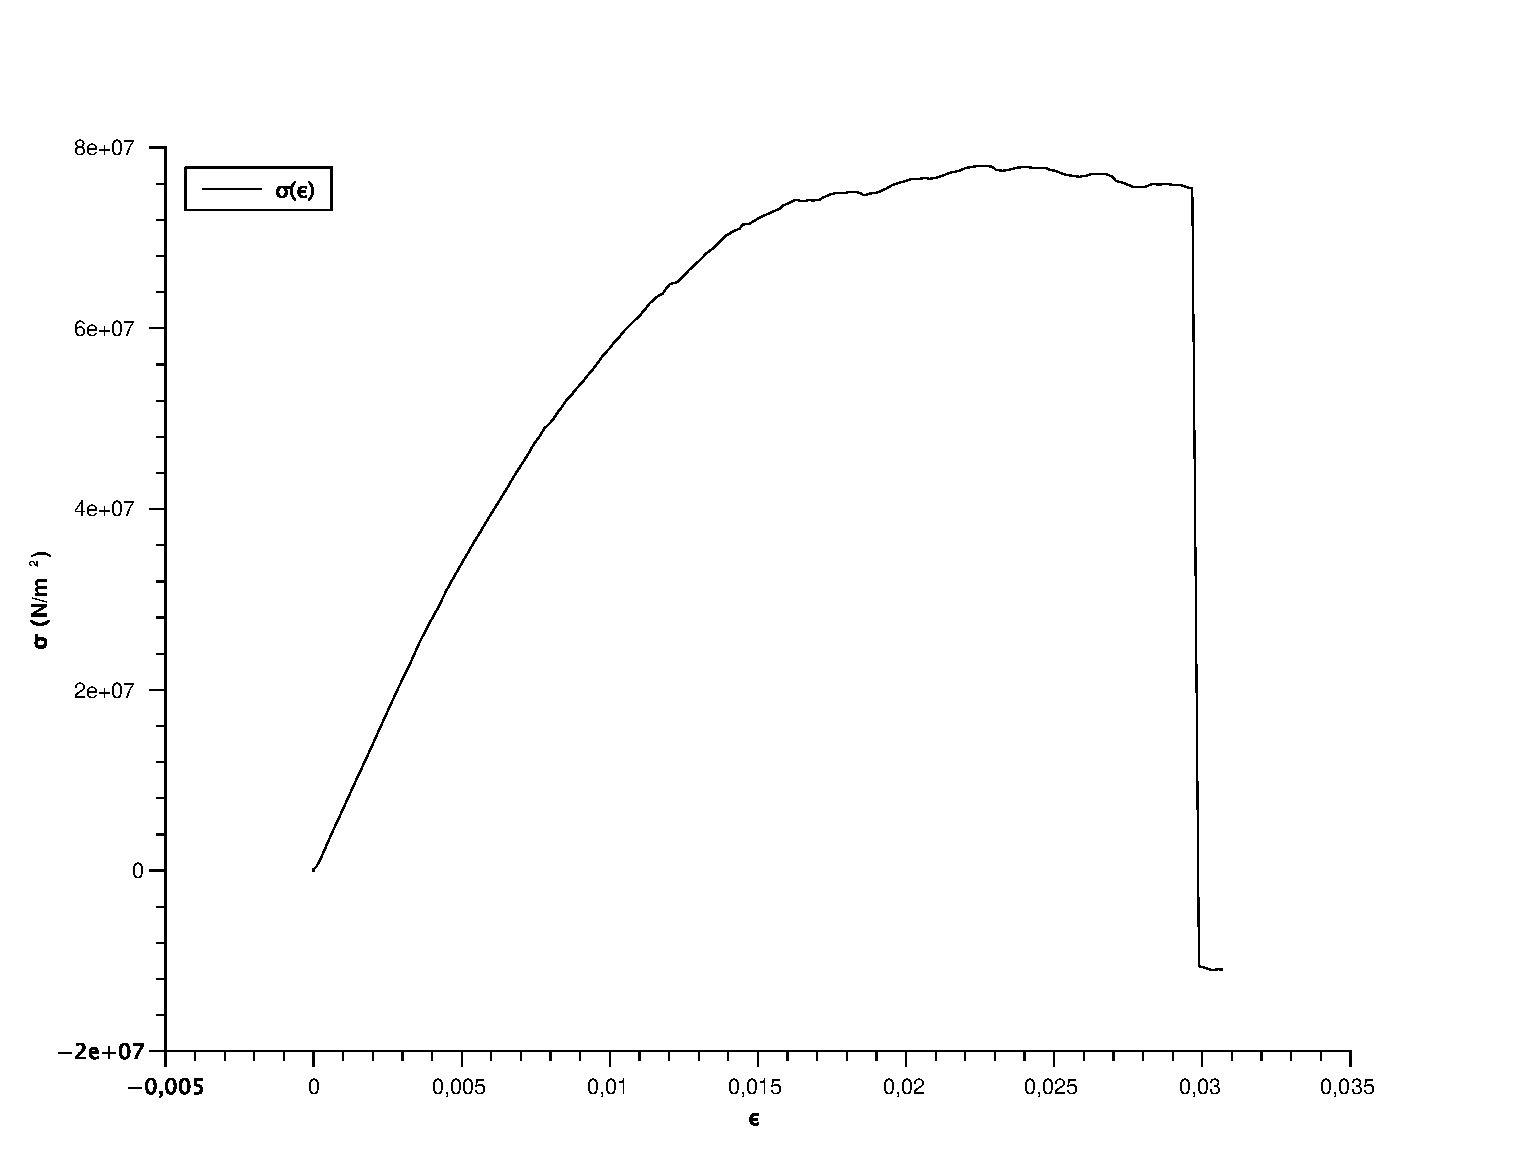
\includegraphics{Tensile/tensileAcrylicFastSigma.eps}}
        \caption{$\sigma(\epsilon)$ for acrylic fast}
        \label{fig:tensileAcrylicFastSigma}
    \end{subfigure}
    \begin{subfigure}{0.49\textwidth}
        \resizebox{\textwidth}{!}{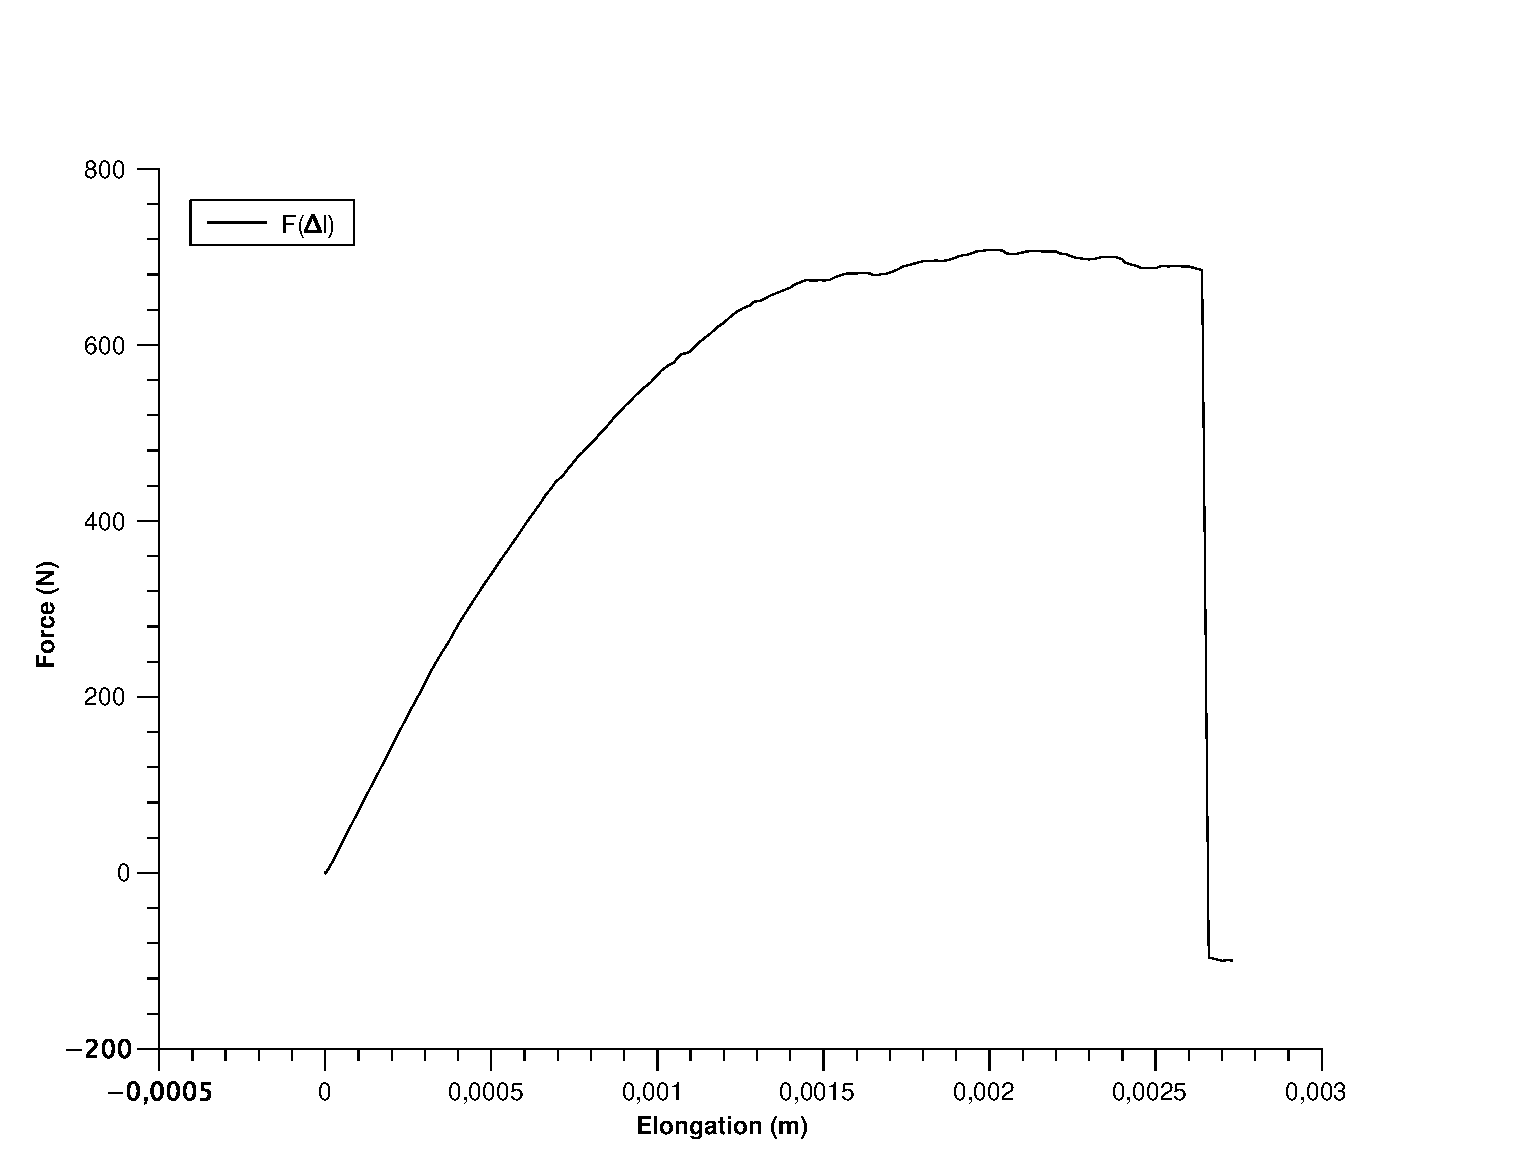
\includegraphics{Tensile/tensileAcrylicFastForce.eps}}
        \caption{F($\Delta l$) for acrylic fast}
        \label{fig:tensileAcrylicFastForce}
    \end{subfigure}
    \caption{Tensile test for acrylic, fast elongation}
    \label{fig:tensileAcrylicFast}
\end{figure}

\begin{figure}[!ht]
    \centering
    \begin{subfigure}{0.49\textwidth}
        \resizebox{\textwidth}{!}{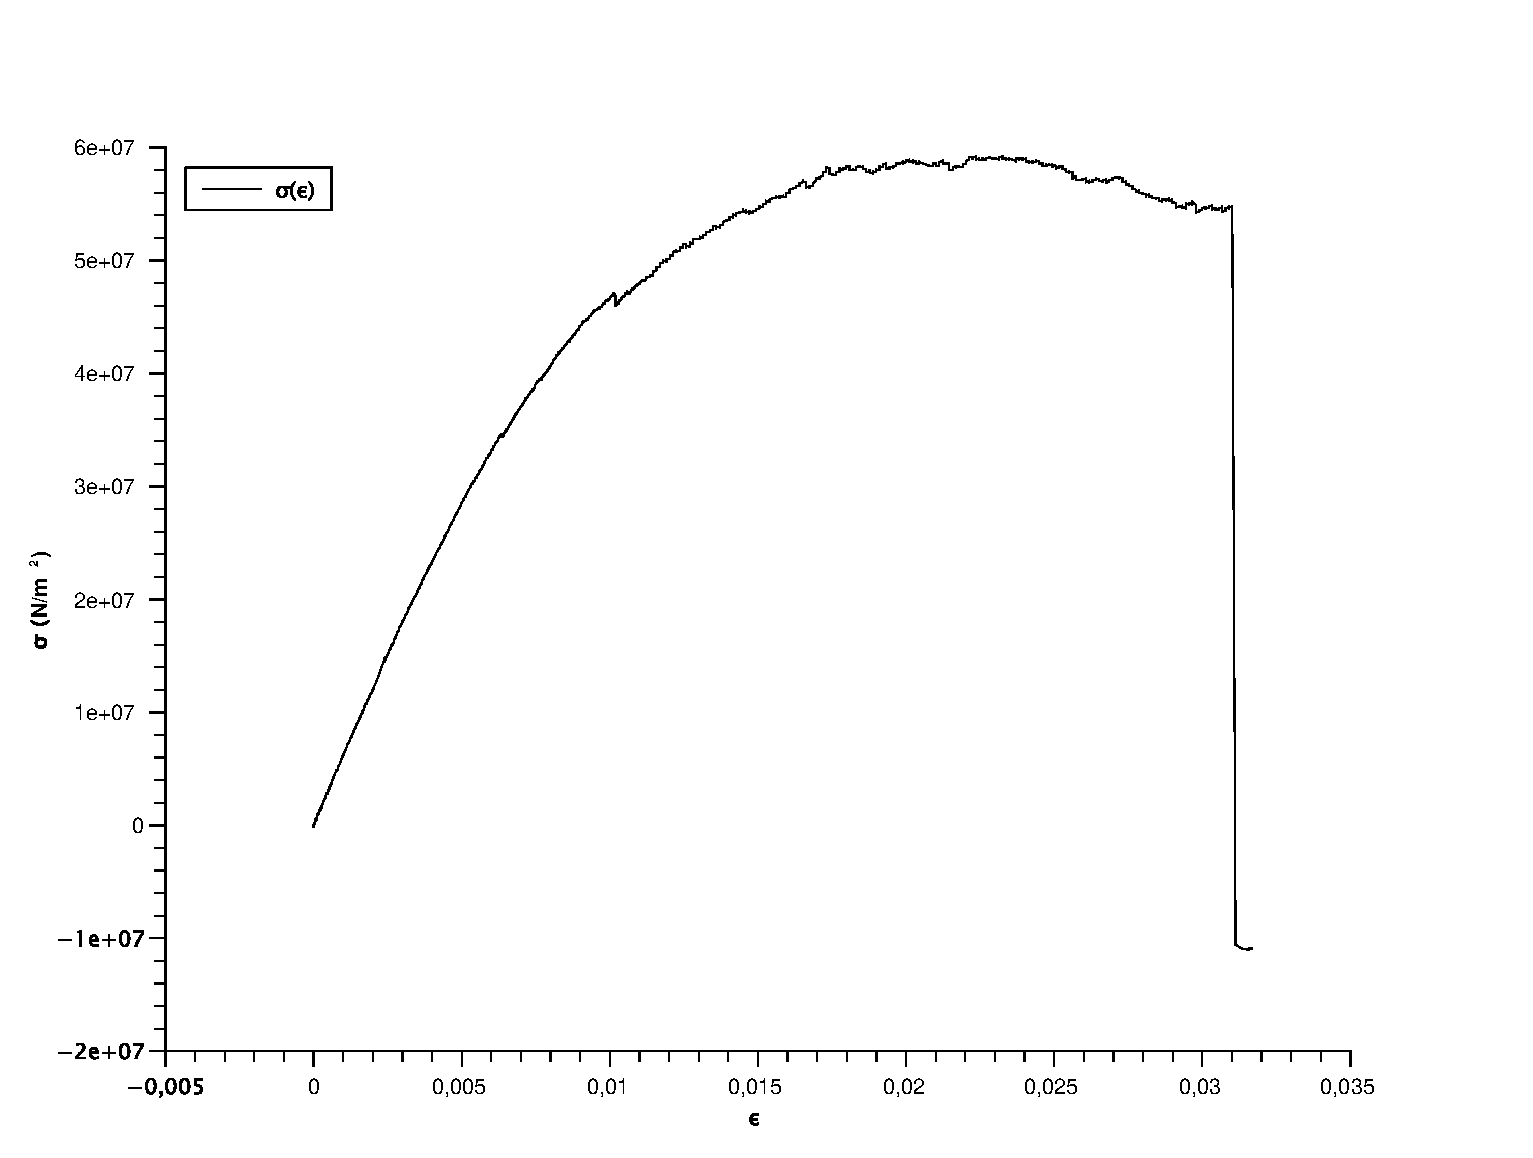
\includegraphics{Tensile/tensileAcrylicSlowSigma.eps}}
        \caption{$\sigma(\epsilon)$ for acrylic slow}
        \label{fig:tensileAcrylicSlowSigma}
    \end{subfigure}
    \begin{subfigure}{0.49\textwidth}
        \resizebox{\textwidth}{!}{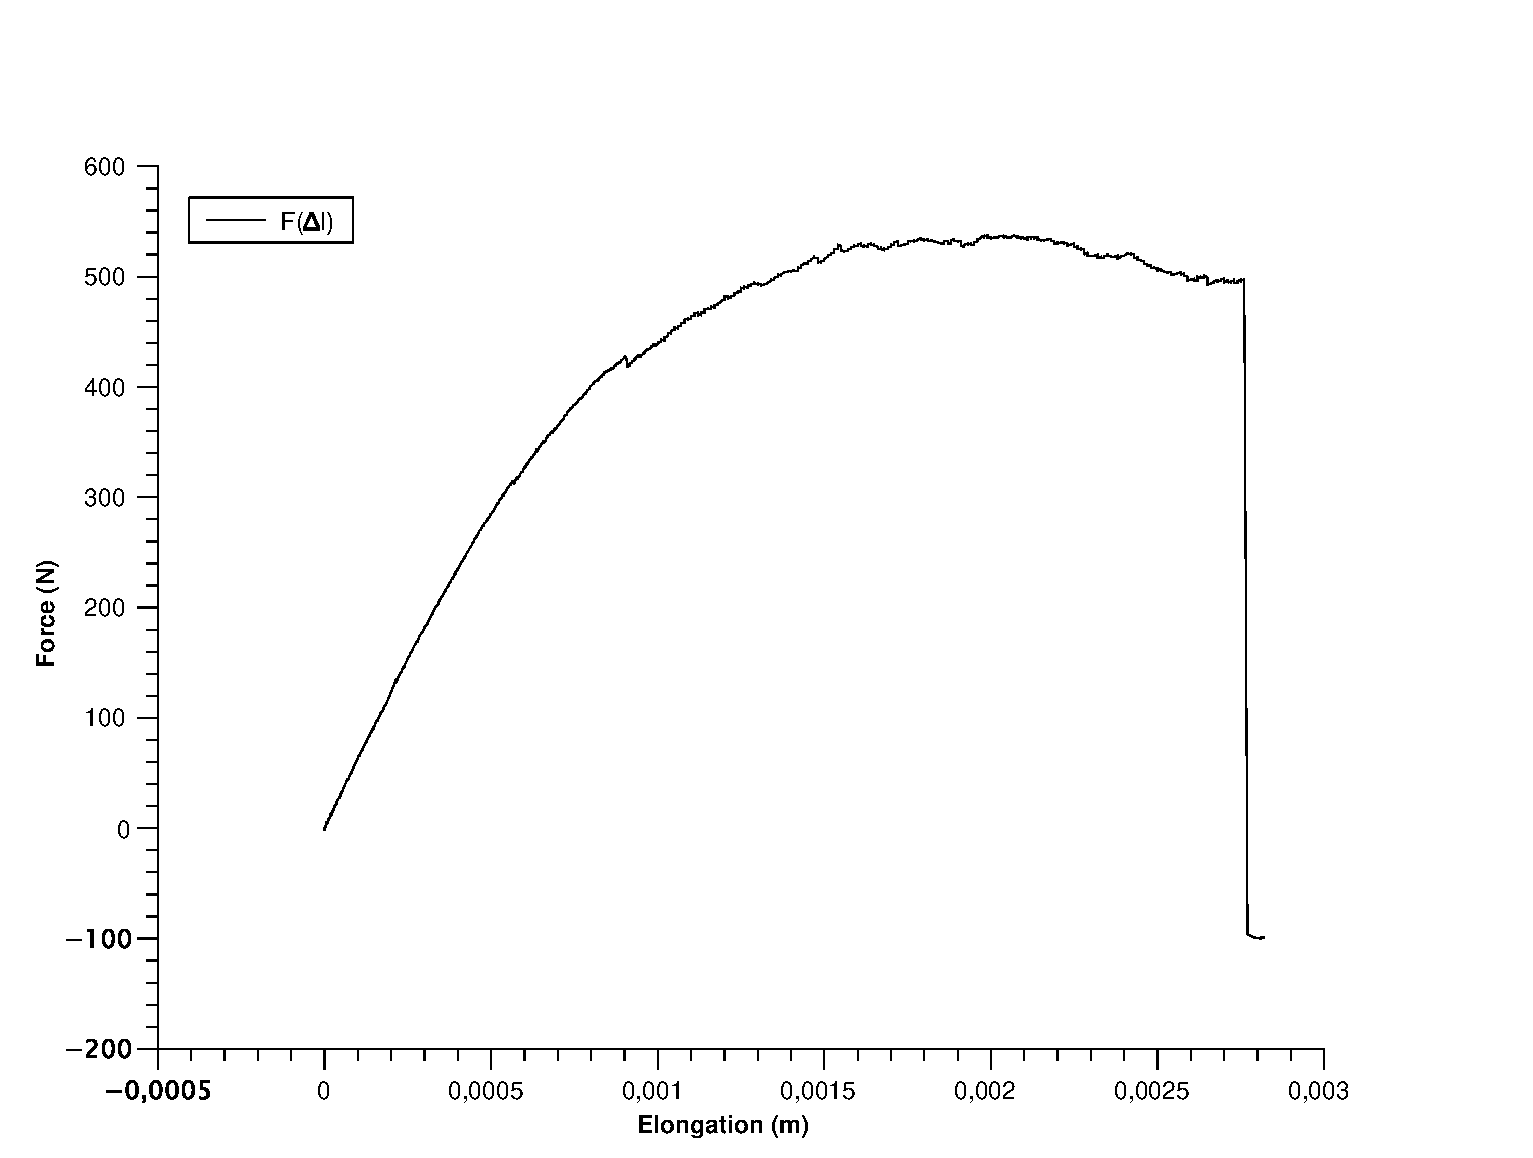
\includegraphics{Tensile/tensileAcrylicSlowForce.eps}}
        \caption{F($\Delta l$) for acrylic slow}
        \label{fig:tensileAcrylicSlowForce}
    \end{subfigure}
    \caption{Tensile test for acrylic, slow elongation}
    \label{fig:tensileAcrylicSlow}
\end{figure}

\begin{figure}[!ht]
    \centering
    \begin{subfigure}{0.49\textwidth}
        \resizebox{\textwidth}{!}{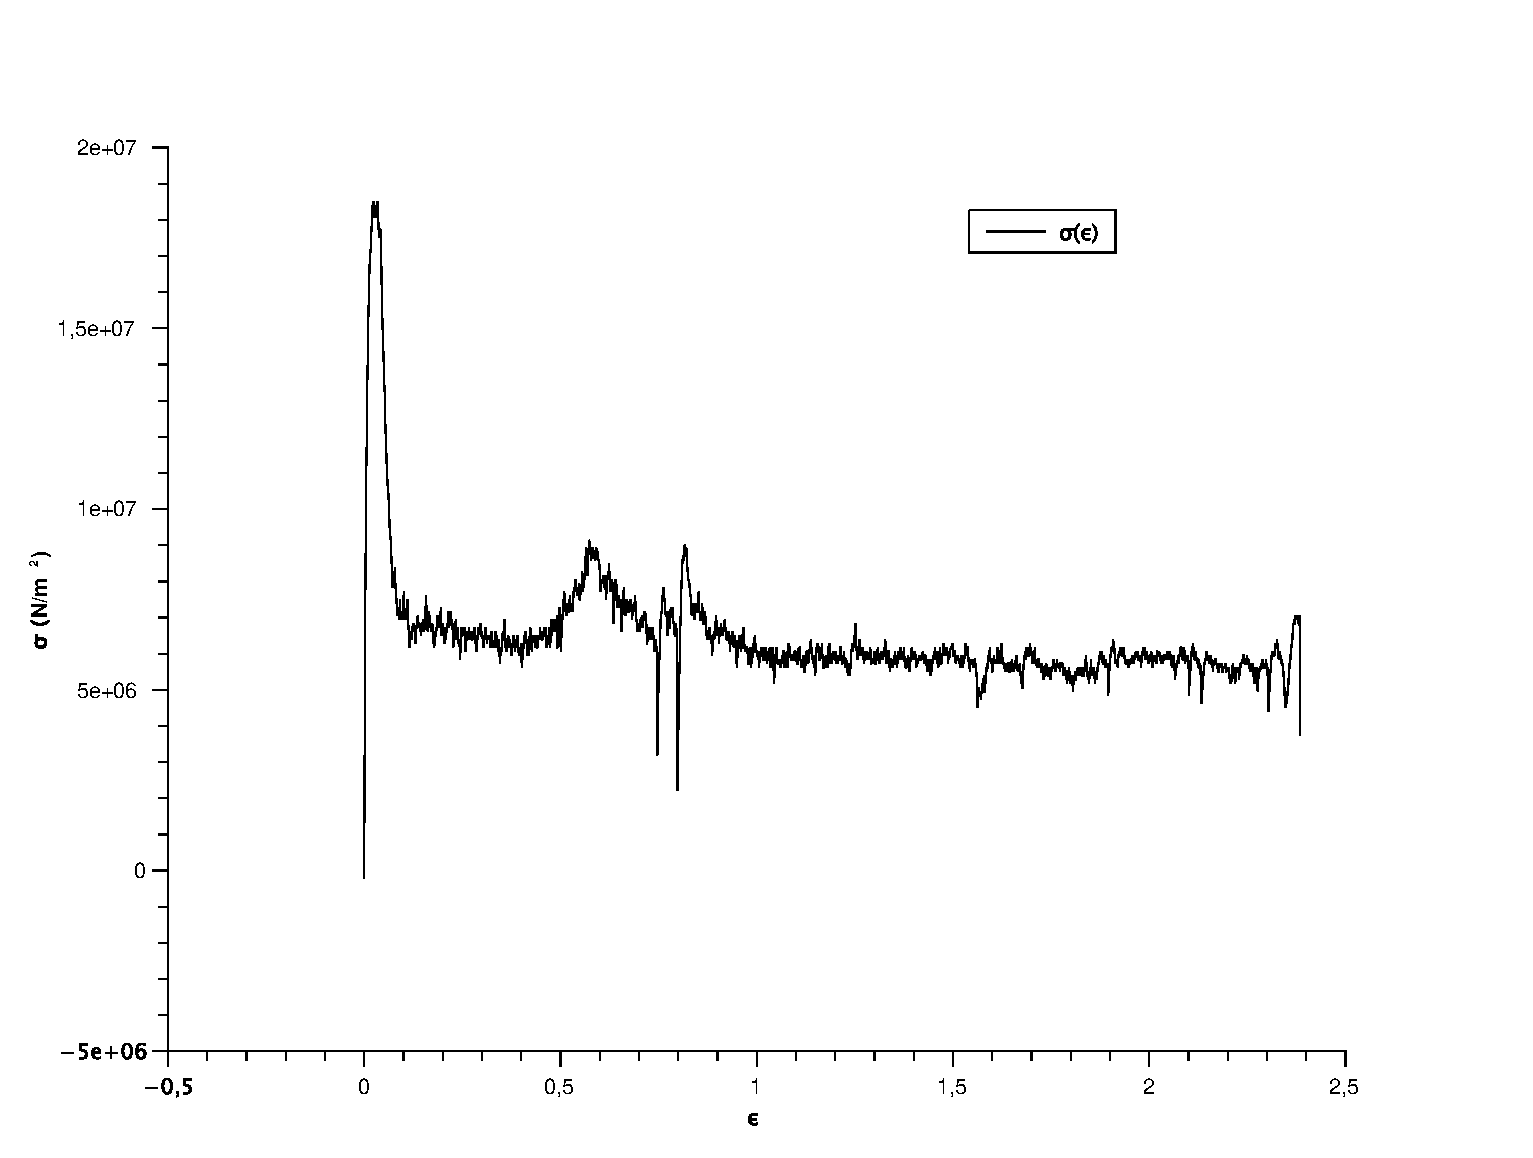
\includegraphics{Tensile/tensilePolyethyleneSigma.eps}}
        \caption{$\sigma(\epsilon)$ for polyethylene}
        \label{fig:tensilePolyethyleneSigma}
    \end{subfigure}
    \begin{subfigure}{0.49\textwidth}
        \resizebox{\textwidth}{!}{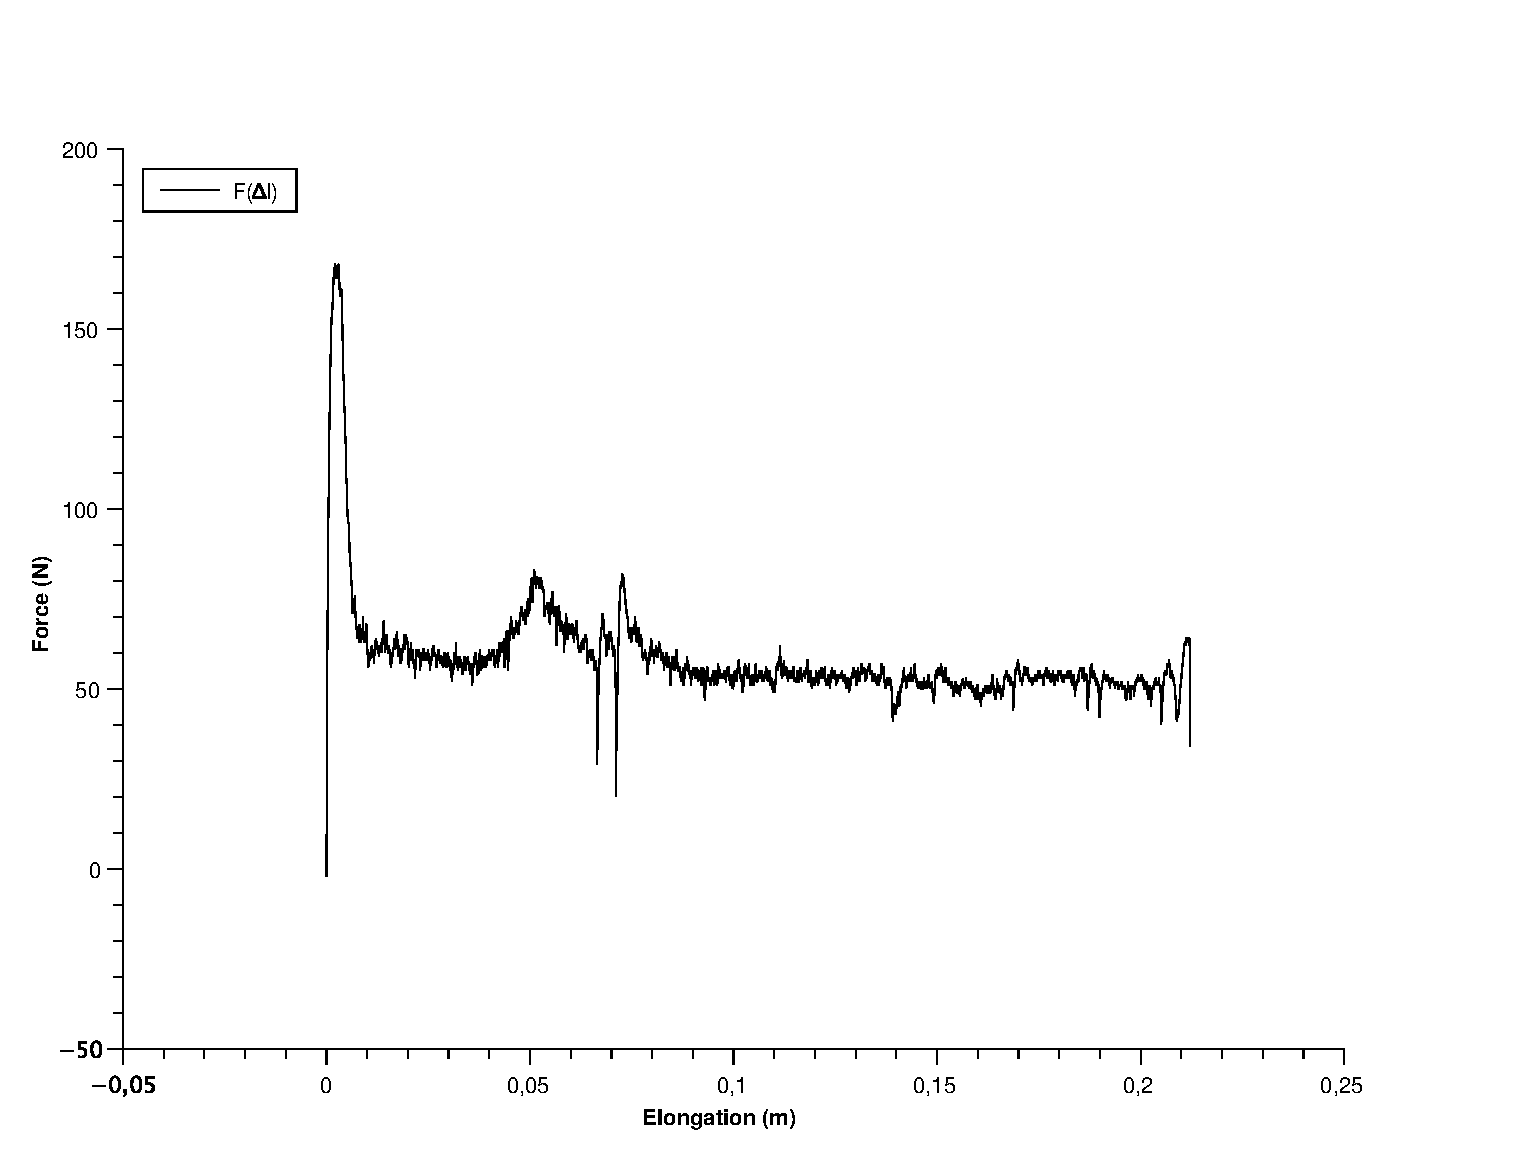
\includegraphics{Tensile/tensilePolyethyleneForce.eps}}
        \caption{F($\Delta l$) for polyethylene}
        \label{fig:tensilePolyethyleneForce}
    \end{subfigure}
    \caption{Tensile test for polyethylene}
    \label{fig:tensilePolyethylene}
\end{figure}
\FloatBarrier

Acrylic bears a striking similarity to metals, but a linear region is not clearly visible. It still deforms elastically though, and barely constricts before breaking. This behaviour happens at both speeds. The impact of speed seems to be that the sample can undergo higher stress, if the elongation happens quickly. The fast sample sustained 712 N, while the slowly stretched sample only 536 N; it is 25 \% less force! The maximum elongation is the same at both speeds.

Polyethylene tensile test gives interesting results. It is very different from the metals and acrylic, as it undergoes necking. When stretch out, the sample becomes thinner, but doesn't break. It undergoes several phases of yielding, softening cold drawing and hardening. The maximum elongation for which it reacts elastically is very small however.

\begin{figure}[!ht]
    \centering
    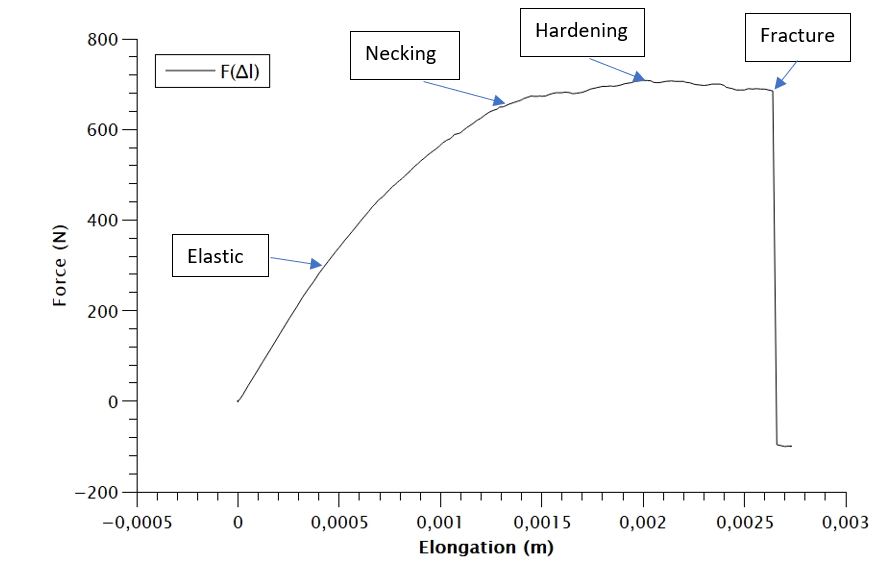
\includegraphics[width=0.6\textwidth]{Tensile/annotated_acrylic(1).png}
    \caption{Regions for an acrylic sample}
    \label{fig:annotated_acrylic}
\end{figure}
\FloatBarrier

\subsection{Shear test}
A calibration of the apparatus is not required, as we don't measure elongation, just force. Shear (aka tangential stress) $\tau$ is defined as \begin{equation}
    \tau = \frac{F}{A}
\end{equation} Where $F$ is the force applied tangentially to the surface $A$. Since the rods are cylinders, this cross-section is a disc. We can determine the shear strength as the highest stress endured during the shearing process. We record the force during the shearing, as seen in figure~(\ref{fig:shearTest})

\begin{figure}[!ht]
    \centering
    \begin{subfigure}{0.32\textwidth}
        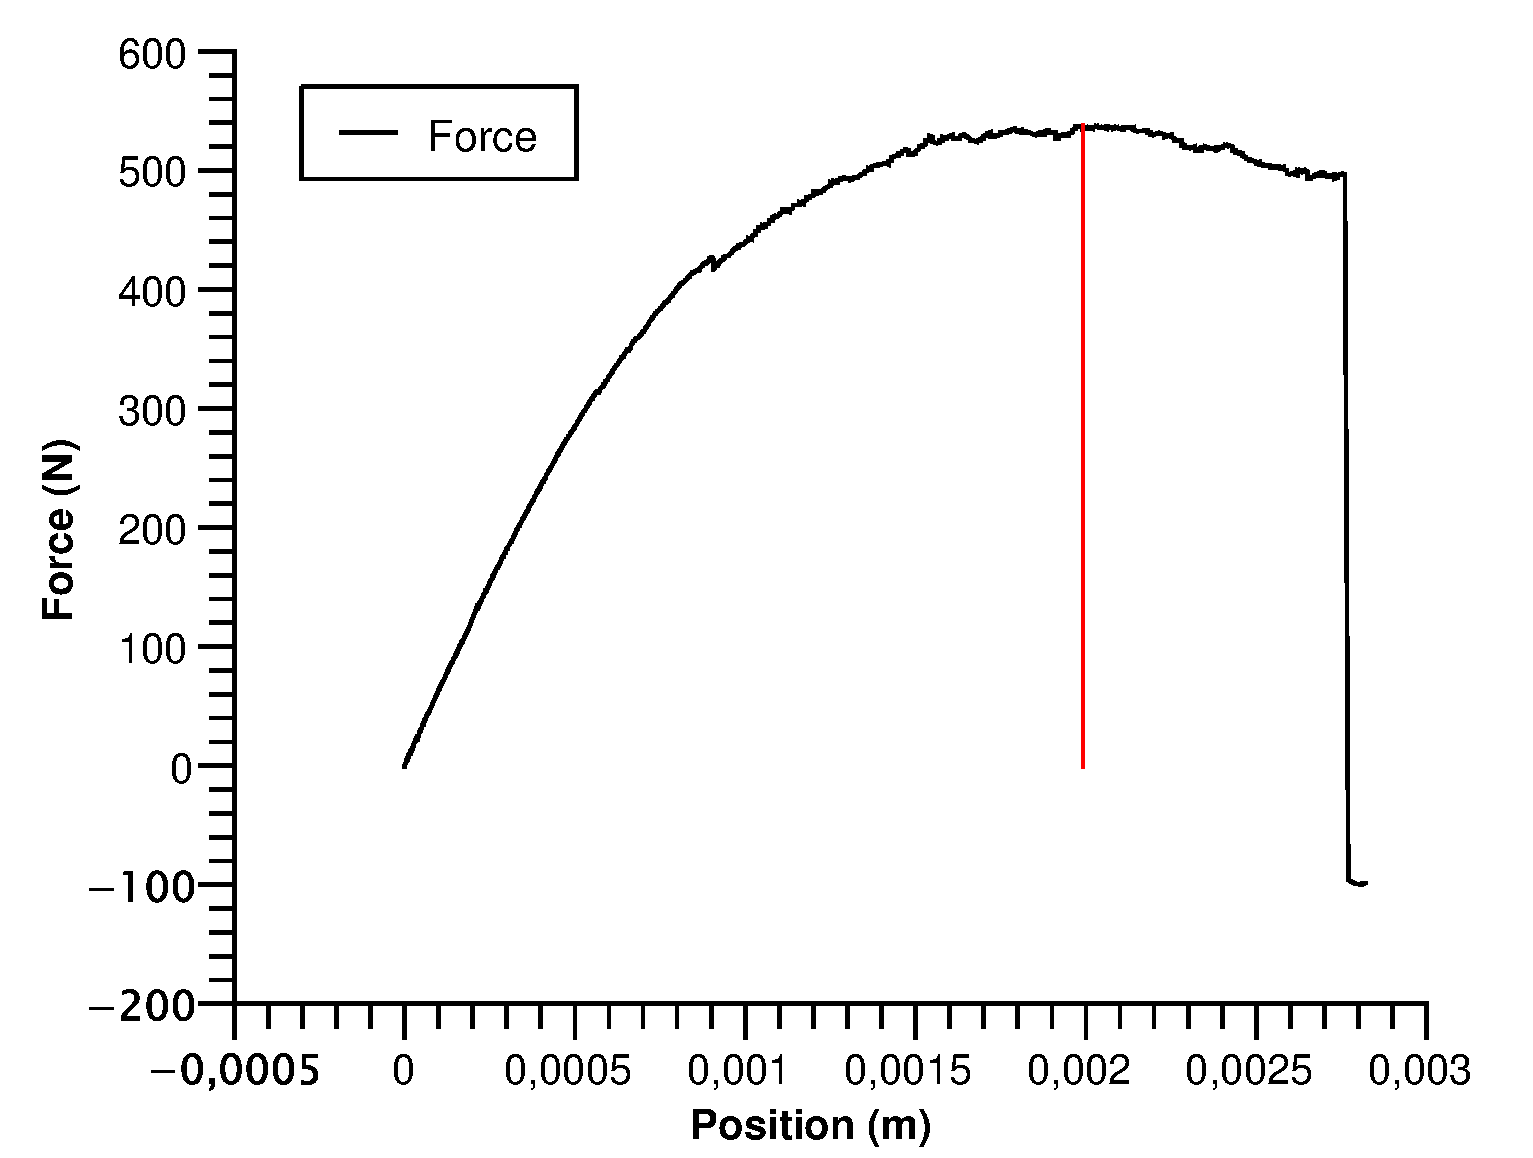
\includegraphics[width=\textwidth]{Shear/ShearBrass.eps}
        \caption{F($\Delta$l) for brass}
        \label{fig:shearBrass}
    \end{subfigure}
    \begin{subfigure}{0.32\textwidth}
        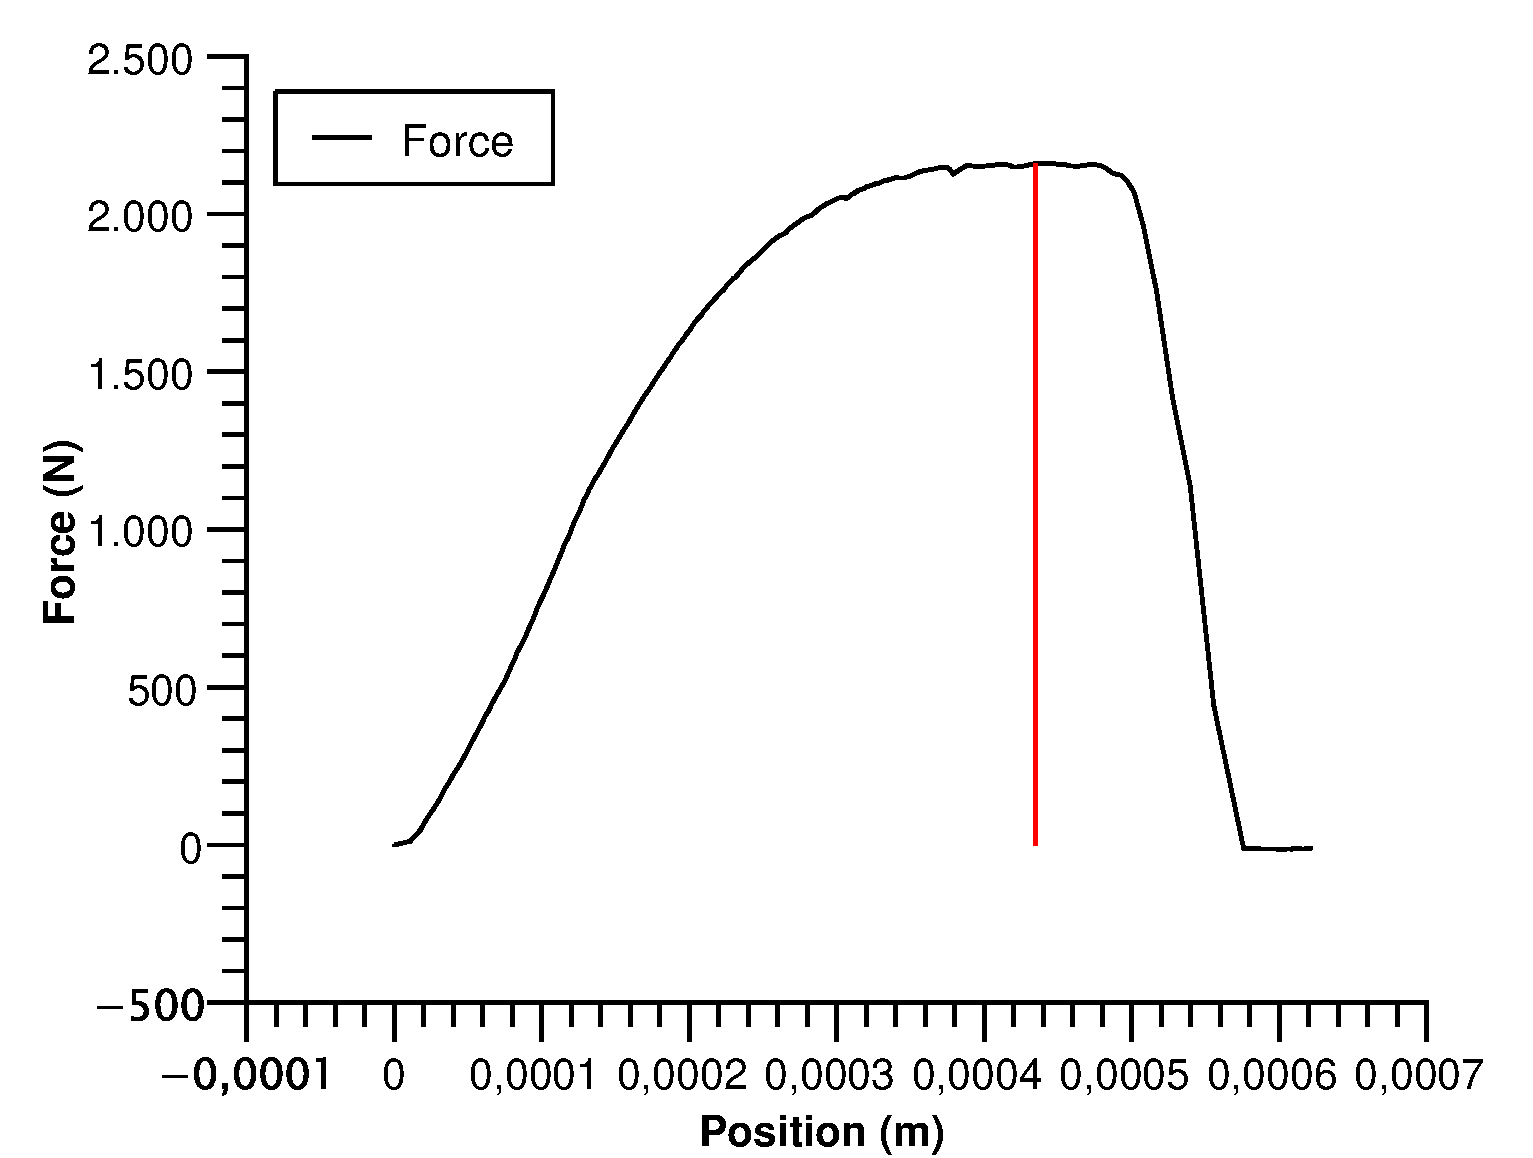
\includegraphics[width=\textwidth]{Shear/ShearAlu.eps}
        \caption{F($\Delta$l) for aluminium}
        \label{fig:shearAlu}
    \end{subfigure}
    \begin{subfigure}{0.32\textwidth}
        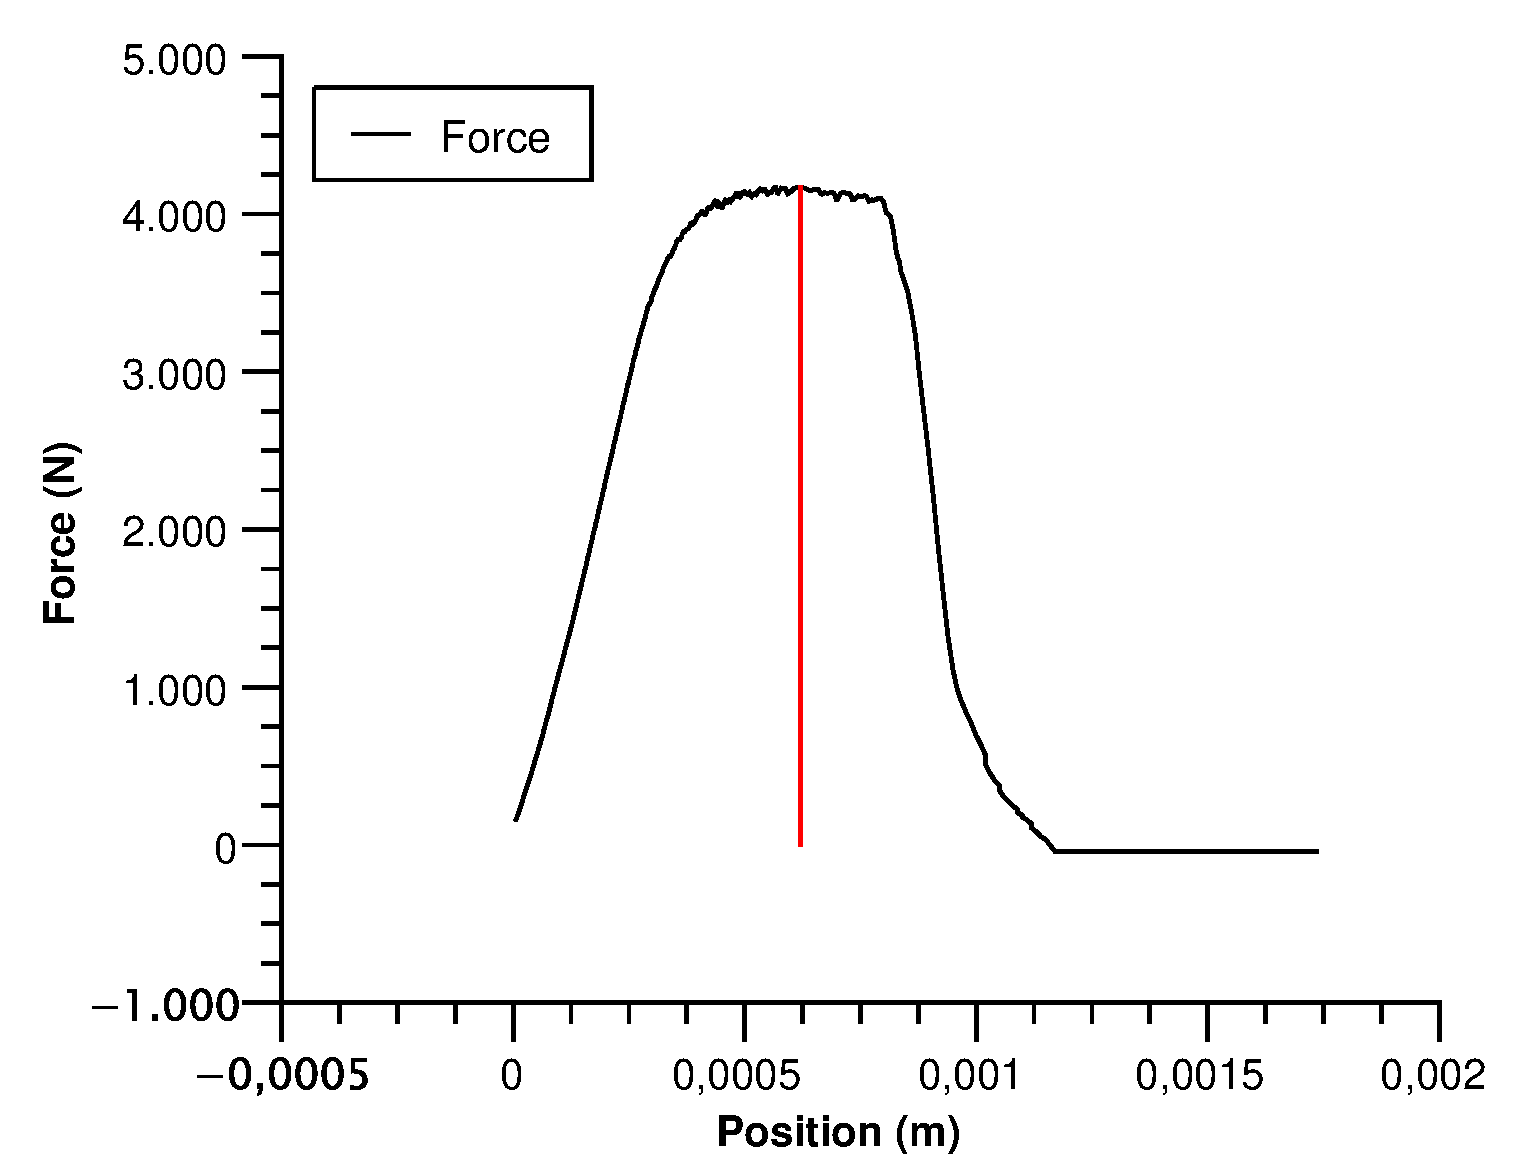
\includegraphics[width=\textwidth]{Shear/ShearSteel.eps}
        \caption{F($\Delta$l) for steel}
        \label{fig:shearSteel}
    \end{subfigure}
    \caption{Shear tests of various material samples}
    \label{fig:shearTest}
\end{figure}
\FloatBarrier

The vertical red lines indicate the position of the highest recorded force. For all materials, the maximum endured stress occured after the linear region, where they were already permanently deformed. The measured values for maximum force and stress can be found in table~(\ref{tab:shearStrength}).

\begin{table}[!ht]
    \centering
    \begin{tabular}{c|c|c}
        material & max. force (N) & max. stress (Nm$^{-2}$)\\ \hline
        brass & 538 & 59.25 $\cdot 10^{6}$ \\
        aluminium & 2160 & 237.9 $\cdot 10^{6}$ \\
        steel & 4169 & 459.1 $\cdot 10^{6}$
    \end{tabular}
    \caption{Maximum force and maximum stress undergone by the material samples}
    \label{tab:shearStrength}
\end{table}

We can also determine the shear strength to tensile strength ration of our samples. This value is predicted by theory to be $\approx 0.6$. For brass we get a ratio of 0.13, for aluminium of 0.55, and for steel a ration of 0.83. Except for aluminium, there is a substantial difference to the theoretical value.

\subsection{Three point bending}
The deflection $h$ formula gives us a way to determine the flexural elastic modulus $E$: \begin{equation}
    h(F) = \frac{l^3 F}{12 \pi R^4 E}
\end{equation} where $R$ is the diameter of the rod, and $l$ the distance between the two outer bending points. When measuring the deflection, we obtained linear curves of the shape $h(F) = s \cdot F$, where s is the slope of the curve (see figure~(\ref{fig:3ptBending})). We can then determine the flexural modulus with: \begin{equation}
    E = \frac{l^3}{12 \pi R^4 s}
\end{equation}

\begin{figure}[!ht]
    \centering
    \begin{subfigure}{0.32\textwidth}
        \resizebox{\textwidth}{!}{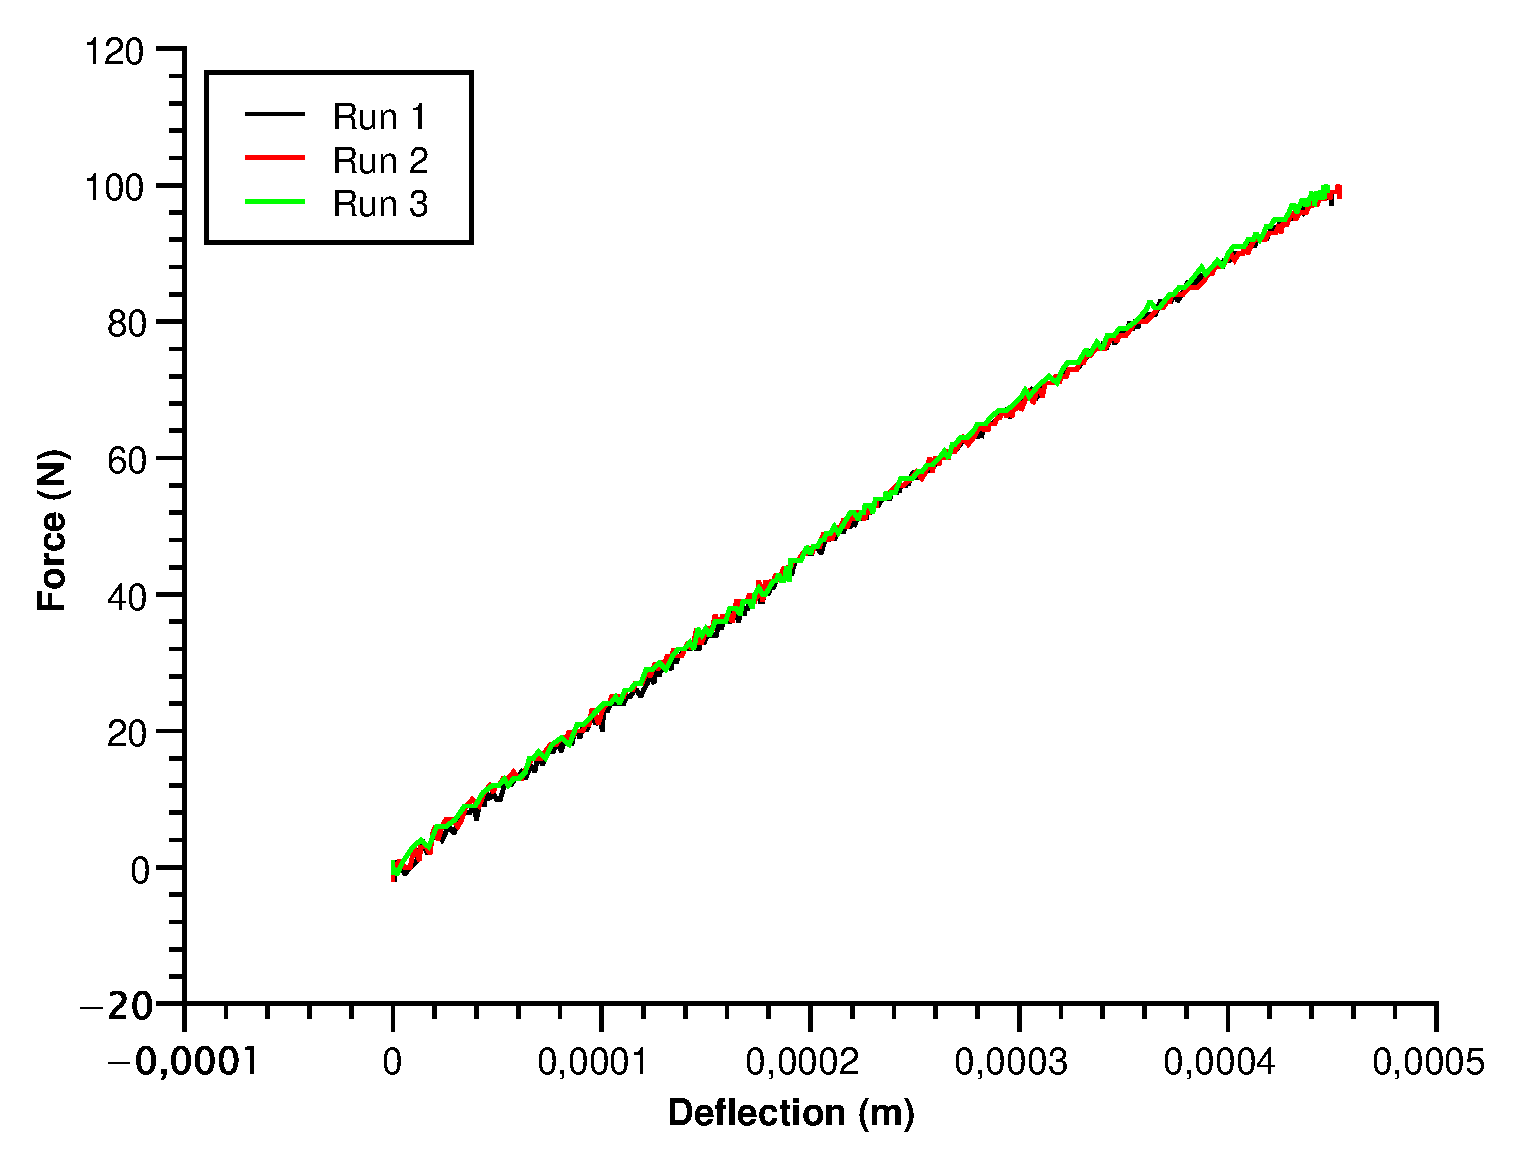
\includegraphics{3ptBending/BrassGraph.eps}}
        \caption{3 point bending test for brass}
    \end{subfigure}
    \begin{subfigure}{0.32\textwidth}
        \resizebox{\textwidth}{!}{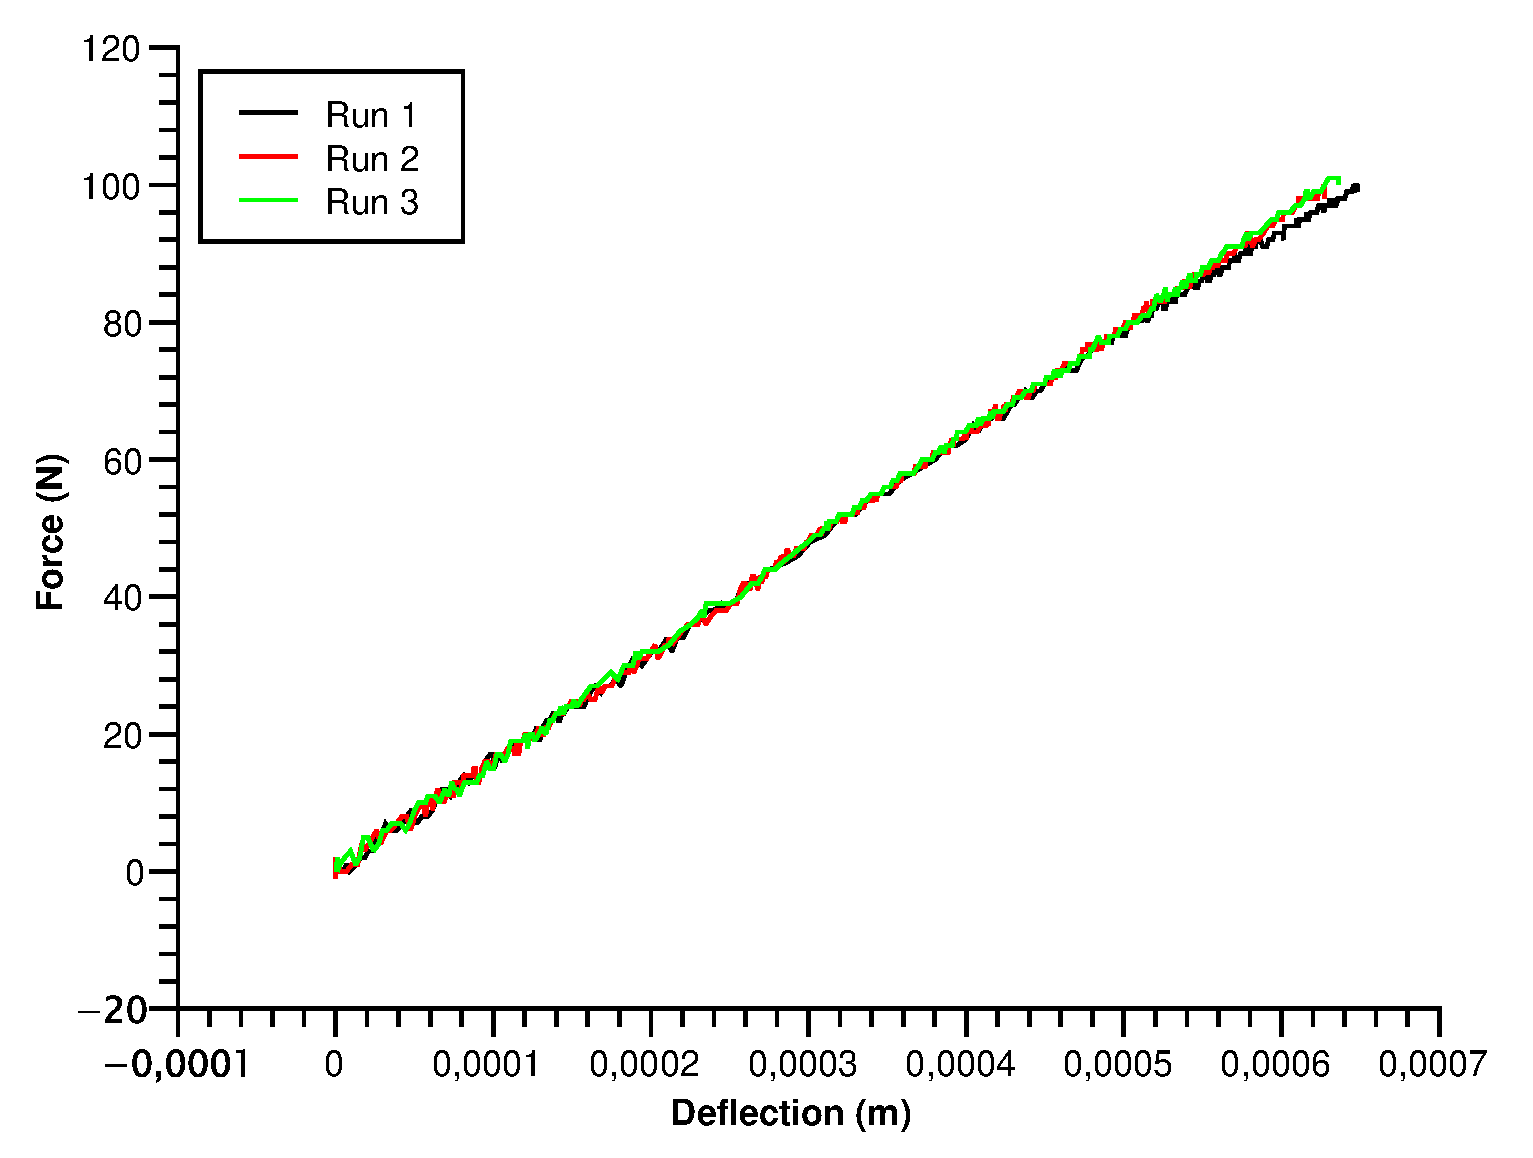
\includegraphics{3ptBending/AluGraph.eps}}
        \caption{3 point bending test for aluminium}
    \end{subfigure}
    \begin{subfigure}{0.32\textwidth}
        \resizebox{\textwidth}{!}{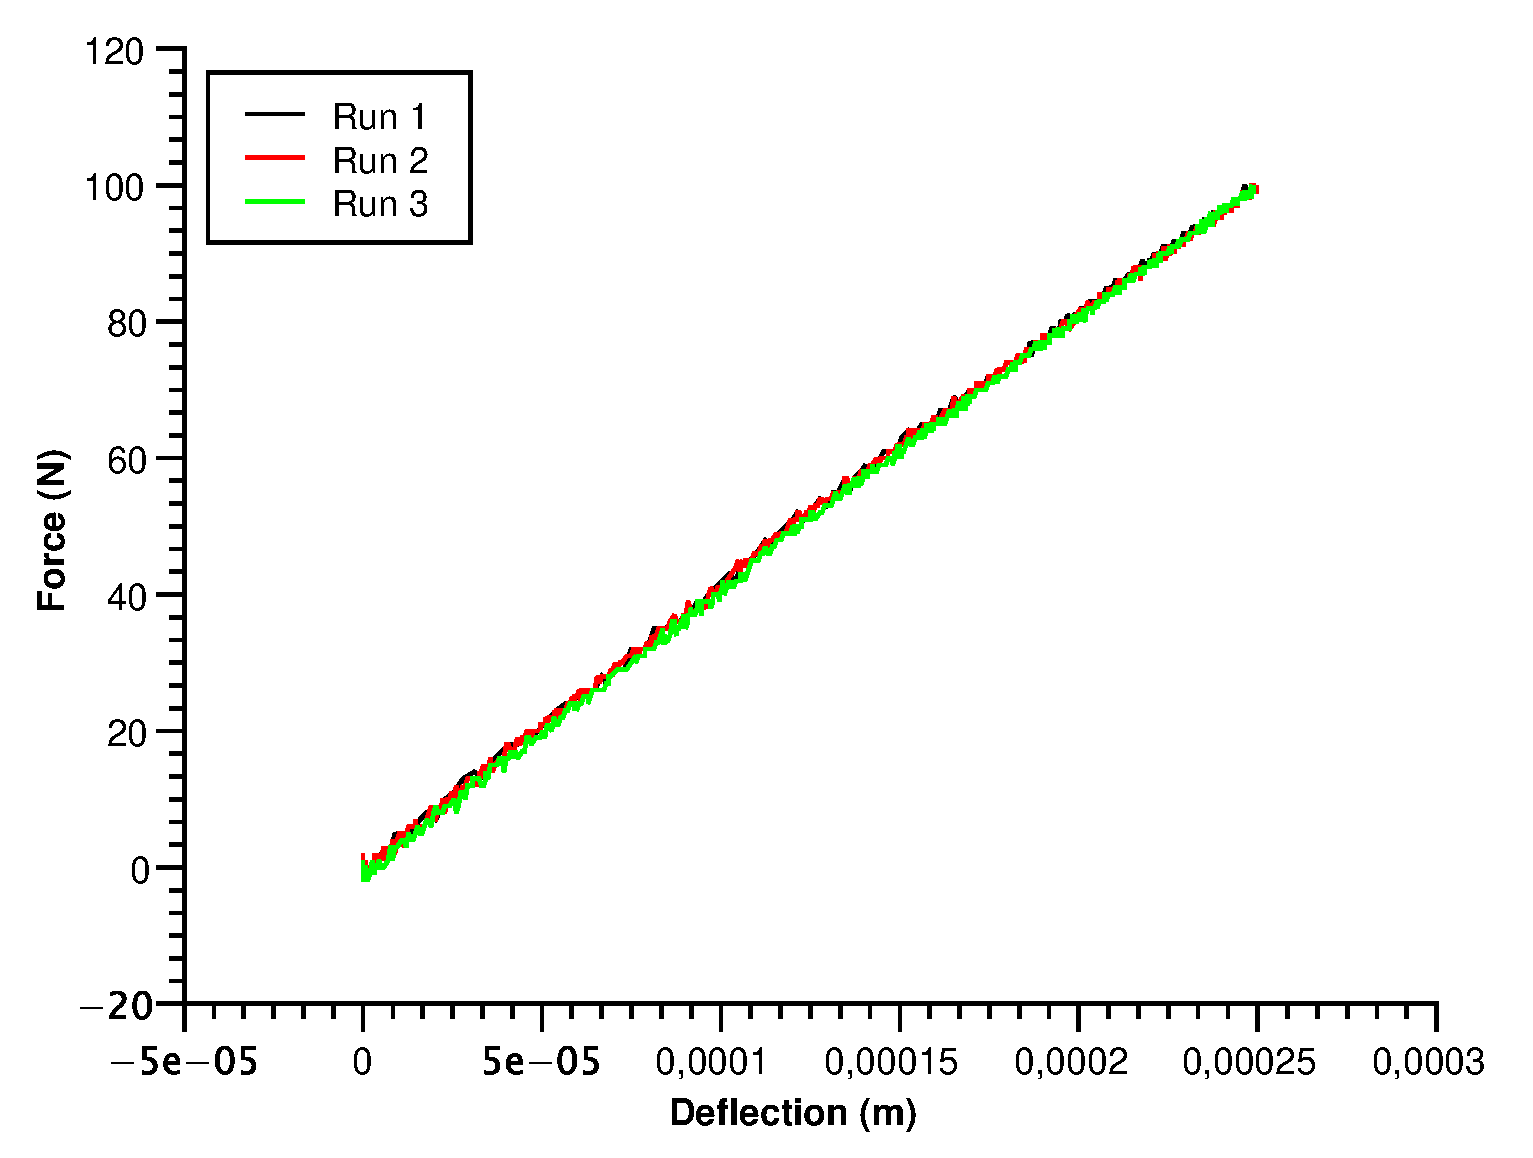
\includegraphics{3ptBending/SteelGraph.eps}}
        \caption{3 point bending test for steel}
    \end{subfigure}
    \caption{3 point bending tests of various materials}
    \label{fig:3ptBending}
\end{figure}
\FloatBarrier

We repeat the experiment 3 times to increase the precision, and obtain following (average) values:

\begin{table}[!ht]
    \centering
    \begin{tabular}{c|c|c}
        Material & Slope & Flexural modulus (Nm$^{-2}$)\\ \hline
        Steel & 403675.6 & $6.7477103 \cdot 10^{-13}$ \\
        Aluminium & 157772.4 &  $1.72646561 \cdot 10^{-12}$\\
        Brass & 155600.7 & $1.75056168 \cdot 10^{-12}$
    \end{tabular}
    \caption{Values of the slope and flexural modulus of various materials}
    \label{tab:my_label}
\end{table}

Note that we set $l = (44.10 \pm 0.05)$ mm, and the diameter of the rods is $2R = (3.40 \pm 0.05)$ mm.

The values of the flexural modulus are much smaller than the values of Young's modulus, the difference is of the order of magnitude of $10^{22}$.

\subsection{Photoelasticity}
For this part, we will be using the 4 point load anvil. With the polarizers, we will be able to see the fringes (as explained in the theory). We notice that fringes appear at the contact point of the anvils, an area where there is high stress. In order to analyse this behaviour, we write down the applied force whenever a new fringe appears. 
\begin{figure}[h]
    \centering
    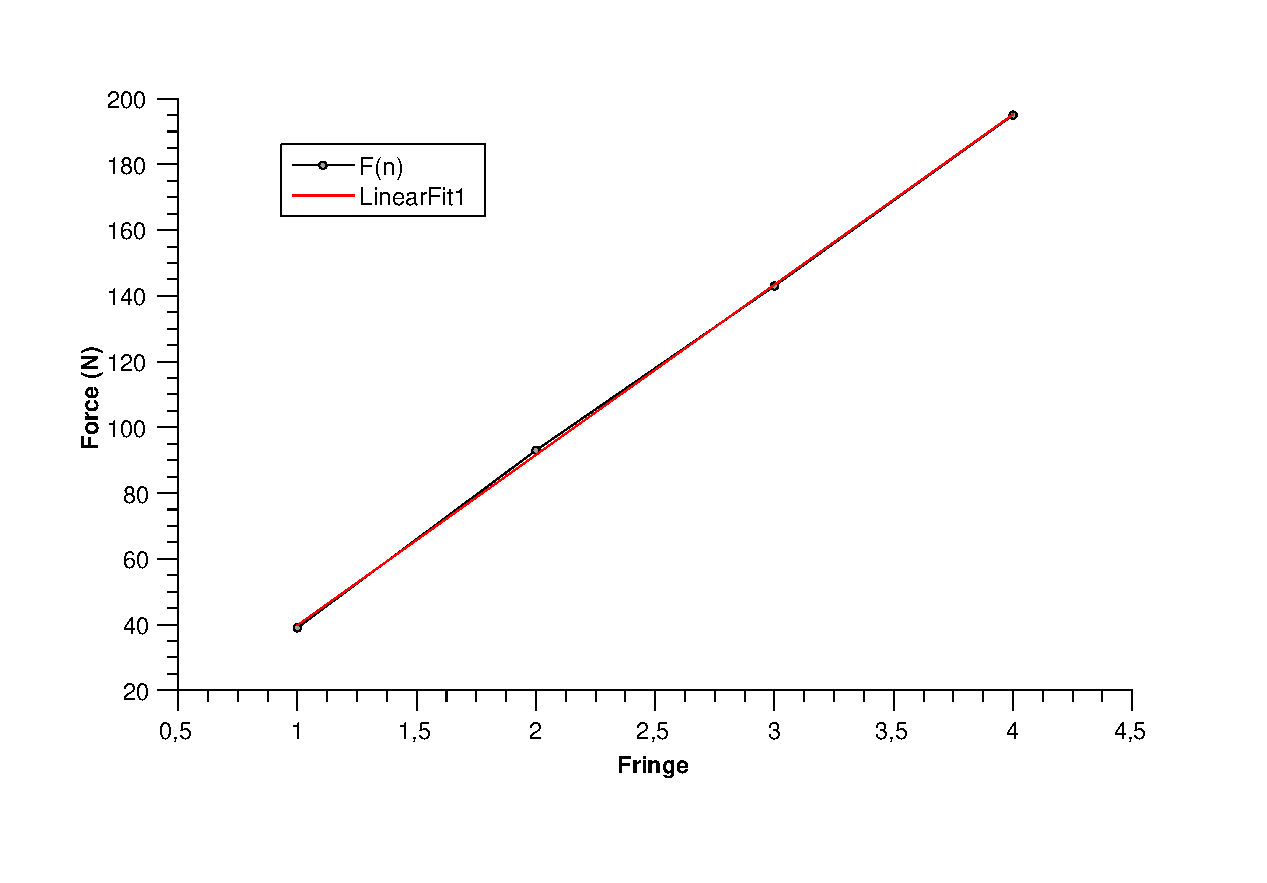
\includegraphics[width=0.7\textwidth]{Photoelasticity/fringes.eps}
    \caption{Force as a function of amount of fringes}
    \label{fig:photoelasticity}
\end{figure}
As the fringes are hard to determine, because it is hard to distinguish if a new line has appeared, we only have 4 data points. As a result we get a nearly linear slope, which means that there is some sort of proportionality between the amount of fringes (n) and the applied force.
The resulting slope is:
\[\ slope =  51,8 \pm 0,5  \ N/n \]\
%Unit??

\section{Conclusion}
With this experiment, we were able to learn of mechanical properties of various materials such as metals and polymers. In this experiment we have studied the tensile and shearing properties, as well as the behaviour under 3 point bending of various metals and polymers, and examined the photoelastic effect. We determined experimentally Young's modulus, the tensile and shear strength and flexural modulus of our samples. We then determined the relationship between acted force upon a material, and the resulting fringes under polarized light to be linear.


\printbibliography

\end{document}
